\documentclass[a4paper,11pt]{report}
\usepackage{geometry}
\geometry{verbose,a4paper,tmargin=25mm,bmargin=25mm,lmargin=25mm,rmargin=25mm}
\usepackage[utf8]{inputenc}
\usepackage[singlespacing]{setspace}
\usepackage{textcomp}
\usepackage{blindtext}
\usepackage{titlesec}
\setlength{\marginparwidth}{2cm}
\usepackage{todonotes}
\usepackage[ngerman]{babel}
\usepackage{listings}
\usepackage{parskip}
\usepackage{verbatim}
\usepackage{graphicx}
\usepackage{chngcntr}
\usepackage{csquotes}
\usepackage[backend=bibtex,citestyle=verbose-ibid]{biblatex}
\usepackage{footnote}
\usepackage[section]{placeins}
\usepackage{algpseudocode}
\usepackage{algorithm}
\usepackage{array}
\usepackage{threeparttable}
\usepackage{pgfplots}
\usepackage{longtable}
\usepackage[automake,acronym,xindy,toc]{glossaries}
\usepackage{hyperref}
\usepackage[ngerman]{cleveref}
\usepackage{makeidx}   % load package



\newcommand*{\bildquelle}[1]{\par\raggedleft\footnotesize Quelle:~#1}


%\newglossaryentry{Canvas}
%{
%name=Canvas,
%description={oder Leinwand. Bezeichnet eine Fläche eines Fensters in der Computergrafik, %%in die virtuell gezeichnet werden kann}
%}


\newacronym{hzb}{HZB}{Helmholtz-Zentrum Berlin}


\makeglossaries
\usepackage[xindy]{imakeidx}
\makeindex




%\addbibresource{bibtex.bib}

\counterwithout{figure}{chapter}
\counterwithout{footnote}{chapter}

\titleformat{\chapter}[display]
   {\normalfont\large\bfseries}
   {\chaptertitlename\ \thechapter}{1em}{\large}
\titleformat{\section}
   {\normalfont\large\bfseries}
   {\thesection}{1em}{}
   
\titleformat{\subsection}
   {\normalfont\small\bfseries}
   {\thesubsection}{1em}{}


\title{Abschlussarbeit Master Medieninformatik}
\author{Viola Jertschat}

\bibliography{references/references}{}

\begin{document}


\begin{titlepage}
	\centering
	\includegraphics[width=\textwidth]{images/beuthlogo.eps}\par\vspace{1cm}
	{\scshape\LARGE Beuth Hochschule für Technik \par}
	\vspace{1cm}
	{\scshape\Large Abschlussarbeit Master Medieninformatik\par}
	\vspace{1.5cm}
	{\huge\bfseries mARt: Interaktive Darstellung von MRT Daten in AR\par}
	\vspace{2cm}
	{\Large\itshape Viola Jertschat\par}
	\vfill
	betreut von\par
	Prof. Dr.-Ing. Kristian \textsc{Hildebrand}

	\vfill

% Bottom of the page
	{\large \today\par}
\end{titlepage}

% Motivation

\chapter{Motivation}

- Neurologen sehen sich MRT Scans Bild für Bild an
- Schlaganfälle sind auf Scans sichtbar
- 2D Darstellung bietet oft keine Vorstellung davon, wie groß der Schlaganfallbereich ist


Anwendung:
- Verdeutlicht Größe und Lage
- Macht betrachten der Daten interessanter
- Kann Erfolg von Therapie visualisieren
-> kann zu Lehrzwecken dienen
- Kann helfen dem Patienten zu veranschaulichen
- 


Die Anwendung ist nicht als einsetzbares Produkt zu verstehen sondern eher als Prototyp, der die Nützlichkeit und das Potenzial des Programms beweist.

\section{Einsatz}



\tableofcontents

\listoffigures

\printglossaries

% Motivation

\chapter{Motivation}

- Neurologen sehen sich MRT Scans Bild für Bild an
- Schlaganfälle sind auf Scans sichtbar
- 2D Darstellung bietet oft keine Vorstellung davon, wie groß der Schlaganfallbereich ist


Anwendung:
- Verdeutlicht Größe und Lage
- Macht betrachten der Daten interessanter
- Kann Erfolg von Therapie visualisieren
-> kann zu Lehrzwecken dienen
- Kann helfen dem Patienten zu veranschaulichen
- 


Die Anwendung ist nicht als einsetzbares Produkt zu verstehen sondern eher als Prototyp, der die Nützlichkeit und das Potenzial des Programms beweist.

\section{Einsatz}


% Related works

\chapter{Verwandte Arbeiten}
\label{related}

\section{AR in der Medizin}
% OPs
% Nutzen und Interaktion

In Bereich der Medizin gibt es viele Anwendungsfälle, 

\section{Visualiserung von MRT-Daten in AR/VR}

Auch in AR wurden bereits innere Organe dargestellt, 


\section{Volume Rendering}
% Grundlagen & verwnadte Arbeiten

\chapter{Aktueller Stand der Technik}
\label{grundlagen}
%-------------------------------------------------------------
\section{AR in der Medizin}												 %
%-------------------------------------------------------------
 %// TODO:
 Relevante Arbeiten identifizieren
 genau beschreiben: TEchniken? Unterschiede zu meiner arbeit warum relevant?
 
Der Nutzen, den AR-Anwendungen in der Medizin darstellen wurde bereits von zahlreichen Arbeiten belegt. Die Einsatzbereiche sind dabei vielfältig.
Beispielsweise stellt \footcite{Voinea16} eine AR-Anwendung vor die den Lernprozess im Bereich der Biomechanik unterstützt.

\subsection{Bildgestütze medizinische Eingriffe}

Ein großer Anwendungsbereich ist der Einsatz von AR in der Ausführung und Vorbereitung von Operationen. Bei einem chirurgischen Eingriff kann für den Patienten ein hohes Risiko, eventuell sogar Lebensgefahr bestehen. Deshalb ist es wichtig, dass der operierende Arzt sich bestmöglich auf seine Aufgabe vorbereiten kann, wobei AR-Anwendungen ihn unterstützen können.
Die Kerneigenschaft von AR ist die Fähigkeit der Technologe die Umgebung des Nutzers mit zusätzlichen Informationen anzureichern. Im Rahmen einer Operation bedeutet das Daten und Bildmaterial zum Fall des Patienten anzuzeigen. Um dem Arzt bei der Orientierung während des Eingriffs zu unterstützen ist es sinnvoll ihm anatomische Bilder zur Verfügung zu stellen, die er vorher bereits studiert hat. Diese stammen meist aus zuvor erzeugten MRT-Daten, die unter Umständen weiterverarbeitet wurden. Durch AR können diese in Echtzeit an der realen Positionen angezeigt werden. 
Die folgenden Arbeiten haben sich mit der Umsetzung dieses Konzeptes beschäftigt.

% Hololens

% Andere Hardware
AR-Systeme werden genutzt um MRT-Daten während eines Eingriffs zugänglich zu machen. Während ein Patient sich in einem MR-Scanner befindet, können die MRT-Bilder direkt an den Arzt weitergeleitet werden. Dieser kann diese zur besseren Orientierung bei z.B. Injektionen nutzen. Offene MRT-Systeme (s. \ref{mrt}) ermöglichen dabei eine Abbildung der betroffenen Organe während des Eingriffs. Die Bildqualität ist allerdings deutlich schlechter als bei geschlossenen Systemen. Bei einem geschlossenen System hat der Arzt dagegen während des Scans keinen Zugang zum Patienten. Um einen MRT-gestützen Eingriff durchführen zu können werden die vorher erstellten MRT-Bilder auf den Patienten projiziert. zur Umsetzung eines Systems gibt es verschiedene Ansätze.
In \citet{Fritz2012} wird ein System vorgestellt, bei dem eines transparenten Spiegels MRT-Bilder über einen Patienten bzw. ein Modell projiziert werden. Die Visualisierung soll Ärzte bei der Nadelführung für Injektionen der Wirbelsäule unterstützen. 
\cite{khamene03} verwendet für einen ähnlichen Anwendungsdall ein HMD und projiziert die Bilder abhängig vom Blickwinkel des Arztes auf den Patienten. Das HMD wurde in \cite{khamene01} weiterentwickelt, sodass der Arzt es während einer Gehirnoperation tragen kann. Dabei wird das Körperinnere durch eine dreidimensionale Visualisierung sichtbar gemacht, die aus MRT-Bildern gewonnen wurde. 

Bildgestüzte Operationen 
\cite{fuchs98} verwendet ebenfalls ein HMD. Über dieses werden Bilder aus einer Laparoscopy auf den Patienten projiziert. (Relevanz?)
Image guided surgery :\cite{grimson99} und  \cite{KerstenOertel2013TheSO}
\cite{MISCHKOWSKI2006478}
\cite{MISCHKOWSKI2006478} untersucht eine Bildschirm basierte AR-Anwendung, die bei Kieferoperationen zum Einsatz kommt. Mit Hilfe der Anwendung kann der Eingriff geplant werden und während der Operation hilft sie dabei, die Position des Kiefers zu überprüfen. 
\cite{Soler04} beschreibt Methoden zur Automatisierung einer dreidimensionalen Visualisierung von MRT-Bildern der Verdauungsorgane. Sowie den Einsatz von AR bei Operationen in diesem Bereich. 
\cite{GasquesRodrigues17} untersucht die Einsatzmöglichkeiten von AR und VR im operativen medizinischen Bereich. Dazu gehört unter anderem die Entwicklung einer AR-Anwendung für die Hololens, die die Ausbildung von Ärzten in Anatomie und Operationen unterstützen soll. 
\cite{Wendt03} entwickelt eine HMD basierte AR-Anwendung, die MRT-Bilder bei Eingriffen auf den Patienten Projiziert. Die Anwendung wurde mit Bildern des Gehirns an einem Kopfphantom getestet.
\cite{Watts17} stellt ebenfalls eine AR-Anwendung vor, die Bilder auf den Körper des Patienten projiziert. Allerdings ein Projektoraufbau verwendet, sodass mehrere Betrachter gleichzeitig die Augmentierung sehen können. Wie in den meisten genannten Arbeiten werden Marker auf dem Patienten angebracht, um das Bild anzupassen.
\cite{Tabrizi15}


\subsection{Visualisierung von medizinischem Bildmaterial}

Neben der Entwicklung von AR-Sytemen, die währen eines Eingriffs verwendet werden können steht im Fokus vieler Arbeiten die Möglichkeiten der dreidimensionalen Visualisierung der Menschlichen Anatomie. Indem ein realitätsgetreues Abbild eines Organs erzeugt wird, können Diagnosen und Behandlungsmöglichkeiten erleichtert werden.

% Lesen, Referenzen?
\cite{Mangina17} stellt einen Ansatz zur Erzeugung dreidimensionalen Modellen des Herzens vor, um diese zu Lernzwecken und zur Vorbereitung auf Operationen zu verwendet. Um den Nutzen der 3D-Modelle zu maximieren werden sie in einer AR- und VR-Anwendung platziert. Die Daten die dem Modell zugrunde liegen stammen aus einem MRT-Scan.Die Arbeit verfolgt demnach ein ähnliches Ziel wie diese. 
Zur Implementierung der Anwendungen wurde die Spiele Engine Unity 3D verwendet (s. Kapite\ref{implementierung}).
Ziel der Anwendung war es eine Interaktive Lernerfahrung zu schaffen, die es dem Nutzer ermöglicht das Herz in seine verschiedenen Komponenten zu zerlegen. Für diesen Anwendungsfall wird ein Mesh des Organs benötigt, das seine Oberfläche abbildet. Die inneren Strukturen sind dabei irrelevant. Hierin unterscheidet sich  die Ansätze der beiden Arbeiten. mARt setzt den Fokus der 3D-Visualisierung auf das Innere des Gehirns.
Auf Grund der Notwendigkeit eines Meshs wurde der Marching-Cubes Algorithmus zu dessen Erzeugung eingesetzt. Dieser wird in Kapitel \ref{grundlagen} erläutert.
\cite{Mangina17_2} untersucht die Möglichkeiten zur Erzeugung eines 3D Models aus MRT-Daten genauer.

Ein weiter Ansatz zur Erzeuggung von 3D-Modellen des Herzens wird in \cite{SORENSEN2001193} beschrieben. Hier soll das Modell ebenfalls in eine VR-Anwendung integriert werden, um von Ärzten als Vorbereitung auf eine operation genutzt werden. 
Auch hier soll ein Mesh des Organs erzeugt werden. Die Generierung soll dabei möglichst automatisierbar sein.  Hierzu werden zuerst die Konturen aus den MRT-Bildern extrahiert. Dies resultiert in ein Gitter aus Konturen die dann algorithmisch durch polygone verbunden werden. 
Für die Anwendung, in der das Modell dargestellt wird wurde ein damals erhältliches VR-System eingesetzt, das mit einem HMD und zwei Controllern funktionierte. 
Durch die Controller wurde eine eine einfache aber intuitive Interaktion umgesetzt. Der Nutzer kann das Modell Vergrößern und rotieren.  

\cite{Calvin01} projiziert 2D und 3D Gehirnbilder aus MRTs auf Kopfphantom für Gehirnoperationen.

%-------------------------------------------------------------
\section{MRT}
\label{mrt}												 %
%-------------------------------------------------------------

Die Abkürzung MRT steht für Magnetresonanztomographie. Das bildgebende Verfahren, das auch Kernspintomografie genannt wird, wird in der Radiologie verwendet, um Abbildungen innerer Organe zu erzeugen. Während der Durchführung einer MRT wird der Patient in ein MRT-System geschoben, das einer großen Röhre gleicht. Er sollte sich für die Dauer des MRTs möglichst wenig bewegen, um klare Bilder zu erhalten.
Es gibt offene und geschlossene MRT-Systeme. Offene Systeme haben die Form eines C, das den Patienten umgibt und werden daher auch C-Systeme genannt. in einem geschlossenen ist der Patient dagegen vollständig von einer Röhre umgeben. Die Bildqualität ist bei geschlossenen Systemen deutlich besser.

\begin{figure}
	\centering
	%https://www.flickr.com/photos/11304375@N07/3081315619/
	\includegraphics[width=0.5\linewidth]{images/mri.jpg}
	\caption{Ein geschlossenes MRT-Gerät. Auf die Liege im vorderen Bereich legt sich ein Patient, der dann während des Scans in die Röhre geschoben wird. }
	\label{img:mri}
\end{figure}
 	
\subsection{Verfahren}

Um die inneren Organe eines Patienten zu visualisieren, werden kleinste Teilchen seines Körpers in Bewegung versetzt, die gemessen werden kann. Im Falle einer MRT handelt es sich dabei um Wasserstoffprotonen. Diese haben eine Eigendrehung um sich selbst, den sogenannten Kernspin. Durch ihre positive Ladung, die durch den Kernspin in Bewegung ist, besitzen die Protonen weiterhin ein eigenes Magnetfeld, welches messbar ist. 
Während einer MRT wird mit einer Hochfrequenz-Spule (HF-Spule), die in dem MRT-System verbaut ist um den Körper des Patienten ein Magnetfeld erzeugt. Die Kernspin-Achsen der Wasserstoffprotonen richten sich an diesem aus. Anschließend wird in das Magnetfeld ein Hochfrequenzimpuls, die Larmorfrequenz eingestrahlt. Durch diesen Impuls findet eine Synchronisation der Protonen statt, wobei einige um 180° gedreht werden. Kurz danach laufen die Protonen wieder auseinander und richten sich wieder am Magnetfeld aus. 
Dadurch, dass alle Protonen in dieselbe Richtung zeigen (phasengleich sind), verstärken sie gegenseitig das Signal, dass sie abgeben. Das Signal wird schwächer, sobald sie wieder auseinander laufen (Dephasierung).
Die Zeit, die die Protonen brauchen, um sich wieder am Magnetfeld auszurichten wird als Relaxtionzeit bezeichnet. Dabei wird zwischen T1- und T2-Relaxtion unterschieden.
Die Relaxionszeit ist dabei abhängig von der Zusammensetzung des umgebenden Gewebes. Das gemessene MR-Signal, das durch diese beeinflusst wird, ist also für verschiedene Gewebearten verschieden stark.
\cite{weishaupt09}

\subsection{Datenverarbeitung}

Mit dem eben beschriebenen Verfahren werden jeweils Werte auf der XY-Ebene erfasst. Um dreidimensionale Daten zu erhalten wird diese XY-Ebene entlang der Z-Achse Verschoben. Das Gehirn wird auf diese Weise in einzelne Schichten unterteilt, von denen jede ein zweidimensionales Bild ist.
Diese Unterteilung in Schichten wird erreicht, indem weitere Spulen verwendet werden, die ein ein zusätzliches Magnetfeld (Gradientenfeld) erzeugen, welches das erste Magnetfeld inhomogen macht. Dementsprechend fällt es zu einer Seite hin ab, was sich durch einen Gradienten, den Z-Gradienten, beschreiben lässt. So kann jeder Z-Schicht eine bestimmte Stärke im Magnetfeld zugewiesen und einzelne Schichten durch die Verwendung bestimmter Frequenzen angeregt werden. In Abbildung \ref{img:zGradient} ist schematisch dargestellt, wie die Schichten entlang des Z-Gradienten hintereinander liegen und eine von ihnen angeregt wird.
Es wird immer nur eine Schicht auf einmal gescannt und verarbeitet.

\begin{figure}
	\centering
	\includegraphics[width=0.3\linewidth]{images/zGradientMrt.png}
	\caption{Darstellung der Schichten während eines MRT-Scans. Links ist der abfallende Z-Gradient zu sehen, daneben drei verschiedene Schichten (Ellipsen). Durch das inhomogene Magnetfeld, kann genau eine Schicht mit einer bestimmten Frequenz angeregt werden. Die ausgewählte Schicht ist hier schraffiert. \cite{weishaupt09}}
	\label{img:zGradient}
\end{figure}


Die X- und Y-Werte einer Schicht repräsentieren allerdings nicht, wie bei einem Bild Koordinaten, die der Anordnung der jeweils betrachteten Punkte in der Welt entsprechen. Stattdessen bildet der X-Wert die Frequenz und der Y-Wert die Phase ab. Wie für den Z-Wert werden auch hier Gradienten gebildet und auf das Magnetfeld gelegt. Der X-Gradient verläuft von links nach rechts und sorgt dafür, dass die Larmorfrequenz in dieser Richtung zunimmt, sodass die jeder Punkt seine eigene Frequenz hat.Der Y-Gradient, der senkrecht verläuft, beeinflusst auf dieselbe Weise die Phasen einer Schicht. Er wird dabei nur kurz nach dem Einstrahlen des Hochfrequenz-Impulses eingeschaltet, wenn sich die Protonen bereits ausgerichtet haben.

Für jeden Punkt gibt es also eine Magnetfeldstärke (Z), eine Frequenz (X) und eine Phase (Y). Diese Werte aller Punkte werden in einer Matrix gespeichert, die K-Raum genannt wird. Die Matrix entspricht allerdings noch nicht der bildlichen Darstellung, die angestrebt wird, da die Werte eine andere Bedeutung haben. ? Deshalb werden sie mit Hilfe der Fouriertransformation in lesbare Bilddaten umgewandelt, die die entsprechenden Organe schichtenweise abbilden. 
\cite{weishaupt09}

\subsection{Abgrenzung CT}
Eine von der Durchführung ähnliche Methode zur Abbildung des Körperinneren, ist die Computer-Tomographie. Die Verfahren unterscheiden sich jedoch. Denn bei einer CT wird der Patient schichtenweise geröntgt. Dh. sein Körper wird mit Röntgenstrahlung beschossen, die je nach Gewebe, auf das sie treffen unterschiedlich stark abgeschwächt werden, was dann gemessen wird. Die so entstandenen "Querschnitte" des Körpers werden anschließend mit Hilfe eines Computers zu einem dreidimensionalen Bild zusammengesetzt. 

Die CT ist deutlich kürzer als eine MRT. Deshalb wird sie oft bei Notfällen verwendet. Allerdings wird der Patient dabei auch der Belastung von radioaktiver Strahlung ausgesetzt ist, die stärker ist als beim normalen Röntgen. Außerdem ist können Weichteile mit einer MRT besser darstellt werden. Sie eignet sich also mehr zur Untersuchung des Gehirns.


\subsection{Datenformate}

MRT-Bilder werden meist in Dateiformaten gespeichert, die in der Medizin üblich sind. Dazu gehören das NIfTI-Format (Neuroimaging Informatics Technology Initiative) sowie das DICOM-Format (Digital Imaging and Communications in Medicine), welches z.B. neben den Bildern auch Patientendaten speichert.

Das NIfTI-Format wurde 2003 von der Data Format Working Group (DFWG) als Alternative zum vorherigen Analyze 7.5-Format entwickelt, das Probleme mit der Orientierung der Daten aufwies. Durch fehlende Informationen, wie die Daten im Raum liegen war oft nicht klar, welche Gehirnhälfte die rechte und welche die linke ist. Deshalb wird im NIfTI-Format in Header festgelegt, wie die Koordinaten der Voxel auf Weltkoordinaten abgebildet sind. Beide Formate werden im Bereich des Neuroimaging verwendet.
Bilderinformationen werden bei ersterem in einer einzigen Daten mit der Endung .nii gespeichert, während Analyze 7.5 die Daten in zwei verschiedenen Dateien abgelegt hat: Einer Header-Datei und einer, die die Volumendaten enthalten hat. Um mit dem Analyze-Format kompatibel zu bleiben besitzen auch NIfTI-Dateien einen 348 Byte Header.
 
Dem Header folgen die Volumedaten des Scans. Es ist möglich bis zu sieben Dimensionen in der Datei abzulegen. Die ersten drei sind dabei für die X-,Y- und Z-Dimensionen des Volumens reserviert.
% https://brainder.org/2012/09/23/the-nifti-file-format/

DICOM bezeichnet nicht nur das Dateiformat in dem medizinische Bilder gespeichert werden, sondern auch legt auch ein Kommunikationsprotokoll zum Austausch von medizinischen Daten fest. Der DICOM-Standart wird in den meisten medizinischen Einrichtungen verwendet, um medizinische Bilddaten zu speichern und auszutauschen.
Der DICOM-Standart besteht aus 16 Teilen.
%https://hpi.de/fileadmin/user_upload/fachgebiete/meinel/papers/Old_Source/TR_Med_Bildverarbeitung.pdf

Wie bereits erwähnt speichert eine DICOM-Datei neben den Bilddaten weitere Informationen. Dazu können eine ID oder der Patientenname zählen, die als Attribute des DICOM-Objektes hinterlegt werden. 
..

%// TODO:
DICOM genauer beshcreiben
Header vergleichen
vorteile nachteilel

MRT-Bilder werden außerhalb des medizinischen Umfelds allerdings auch in anderen Formaten gespeichert. 
Ein Beispiel dafür ist das PVM-Format, das zum Speichern von volumetrischen Daten genutzt wird. Das Format geht davon aus, dass das Volumen aus quadratischen Voxeln besteht und enthält die Voxelwerte und Größeninformationen über das Volumen.
% http://paulbourke.net/dataformats/pvm/

Die Daten können weiterhin in herkömmlichen Bildformaten, wie JPEG oder PNG gespeichert werden. Dabei entspricht dann eine Bilddatei einer Schicht des Scans. 
 
%16 bit int images, pvm ? Standart?

%------------------------------------------------------
\section{Volumendaten}							  	  %
%------------------------------------------------------

Ein wichtiger Aspekt dieser Arbeit ist die dreidimensionale Visualisierung von MRT-Daten. Deshalb soll an dieser Stelle auf einige grundlegende Aspekte und Begriffe im Zusammenhang mit Volumendaten eingegangen werden. Da das Gehirn durch einen MRT-Scan dreidimensional erfasst wird, liegen die MRT-Daten als Volumendaten vor. Die Daten werden durch ein Skalarfeld repräsentiert. Ein Skalarfeld ist ein Sammlung von Skalarwerten, die in einem Raum verteilt sind. Durch eine Funktion kann jedem Punkt im Raum ein Skalarwert zugewiesen werden. Im Fall von Volumendaten handelt es sich um ein dreidimensionales Skalarfeld. D.h. die Skalarwerte sind innerhalb eines Würfels angeordnet für jeden Skalarwert existieren X-, Y- und Z-Koordinaten, die dessen Position beschreiben. 
Diese Punkte aus denen sich der Volumen-Würfel zusammensetzt werden auch Voxel genannt. Ähnlich wie Pixel in zweidimensionalen Bildern stellen sie die kleinsten Teilchen in einem Volumen dar. 
Die Skalarwerte werden auch als Isowerte des Volumens bezeichnet bei MRT-Daten bildet jeder Wert eine Graustufe ab und liegt damit in dem Bereich von 0-255. 
Über das Volumen verteilt haben benachbarte Werte oft ähnliche Isowerte. Eine Gruppe dieser Werte wird als Isofläche bezeichnet. Isoflächen innerhalb eines Volumens entsprechen oft tatsächlichen Oberflächen des darzustellenden Objektes. Durch das Vergleichen benachbarter Werte ist es also möglich Oberflächen von Objekten zu ermittlen (siehe \ref{marchingCubes}). 

Volumendaten werden oft in 3D-Texturen gespeichert. Diese funktionieren auf dieselbe Weise wie 2D-Texturen und entsprechen, wie beschrieben der Vorstellung eines Würfels. Die Textur besitzt Texturkoordinaten in drei Dimensionen und 

Die Verfahren zur dreidimensionalen Visualisierung von MRT-Daten lassen sich in drei Bereiche teilen: Multiplanar Reformation (MPR), Surface Rendering (SR), and Volume Rendering (VR). \cite{Zhang10} In den folgenden Abschnitten werden diese verfahren erläutert.

%------------------------------------------------------
\section{Volume Rendering}							  %
%------------------------------------------------------
%https://developer.nvidia.com/gpugems/GPUGems/gpugems_ch39.html
% Bezug zu Motivation
Wie in Kapitel \ref{motivation} erläutert, sollen die MRT-Bilder, die der Neurologe untersucht in mARt als dreidimensionales Volumen dargestellt werden. Volume Rendering bezeichnet die Darstellung eines dreidimensionalen Volumens, meist durch ein Skalarfeld repräsentiert, auf einer zweidimensionalen Bild. MRT-Bilder, die in Graustufen vorliegen bilden ein solches Skalarfeld. 

Dadurch, dass das Volumen aus Voxeln gebildet wird, gibt es keine Oberfläche, die das abzubildende Objekt beschreibt. Die Darstellung erfolgt deshalb anhand eines optischen Modells. Jedem Wert im Datensatz werden dazu optische Eigenschaften zugewiesen, im Allgemeinen Farbe und Opazität. Indem Strahlen durch das Volumen geschossen werden, werden diese Eigenschaften mit einander verrechnet, was schließlich zur Abbildung des gesamten Volumen führt. Diese Technik wird im Abschnitt \ref{rayCasting} genauer beschrieben.
Die optischen Eigenschaften eines Voxels sind abhängig von seinem Isowert, sowie der verwendeten Transferfunktion und dem Shading. 

Im Folgenden werden grundlegende Techniken, sowie verschiedene Verfahren der Umsetzung des Volume Rendering erläutert.

\cite{Kaufman03}
\cite{kniss02}
%//TODO: 
Beispielarbeiten recherchieren, beschreiben
REFERENZEN-> GPU GEMS

\subsection{Klassifikation}

Die Klassifikation von Voxeln bestimmt deren optische Eigenschaften in Abhängigkeit zu ihrem Isowert. Diese beschreiben, die Aufnahme und Abgabe von Licht eines einzelnen Voxels. Die Abgabe von Licht manifestiert sich aus der Sicht des Betrachters in der Farbe eines Voxels. Die Aufnahme äußert sich in dem Grad der Opazität. Durch die Unterschiede in Farbe und Opazität einzelner Voxel, werden verschiedene Bereichen, wie z.B. Gewebestrukturen voneinander unterscheidbar. Die Qualität des gerenderten Bildes hängt zu einem großen Teil von der Klassifikation ab.Oft wird eine Transferfunktion verwendet, um Voxel zu klassifizieren. Auf diese wird im folgenden Abschnitt näher eingegangen. 

Das Ergebnis einer Klassifikation hängt von dem Zeitpunkt ab, zu dem diese durchgeführt wird. Sie kann vor oder nach der Interpolation der Volumendaten durchlaufen werden.

Die Daten müssen interpoliert werden, da das Volumen wie mehrfach beschrieben in einzelnen Werten vorliegt. Der Raum zwischen diesen Werten ist nicht definiert. Um ein zusammenhängendes Volumen darstellen zu können muss also eine Interpolation zwischen den Werten stattfinden. Diese wird in der Regel durch die Verwendung eines Filters bzw. einer Convolution umgesetzt. Sir findet während des Rasterisierungsschrittes statt?

Werden die Voxel vor dieser Interpolation klassifiziert, wird dies als Pre-Klassifikation bezeichnet. Dabei werden jedem Isowert die entsprechenden Eigenschaften zugewiesen. Die Zwischen den Voxeln bestehenden Lücken werden aufgefüllt, indem zwischen den Farb- und Opazitätswerten interpoliert wird. 
Im Gegensatz dazu, werden bei der Post-Klassifakation zuerst alle Skalarwerte durchlaufen und der Bereich zwischen ihnen durch Interpolation der Isowerte überbrückt. Erst danach werden den Werten durch die Klassifizierung Eigenschaften zugewiesen. Der Unterschied besteht also darin, ob die Erzeugung von neuen Werten, die die vorhandenen verbinden auf Basis der Voxelwerte oder der Werte ihrer Eigenschaften stattfindet. \cite{Hadwiger06}



Obwohl die Vorgehensweisen also beinahe gleich sind, führen sie doch zu deutlich unterschiedlichen Ergebnissen. Die Interpolation der Voxeleigenschaften bei der Pre-Klassifizierung führt zu Artefaktbildung, da die lediglich Eigenschaftswerte "gestreckt" werden, ohne die Formen des Volumens zu beachten. Bei der Post-Klassifikation werden die fehlenden Daten anhand der Struktur des Objektes erzeugt. Dies führt zu einer deutlich klareren Darstellung des Volumens. Der Vergleich ist in \ref{img:prepost} veranschaulicht.

\begin{figure}
	\centering
	%http://schorsch.efi.fh-nuernberg.de/roettger/index.php/VolumeRendering/Pre-AndPost-Classification
	\includegraphics[width=0.7\linewidth]{images/prepostclassification.png}
	\caption{Vergleich zweier Volumen Renderings mit unterschiedlicher Klassifizierung. Durch die Verwendung von Pre-Klassifikation (links) entstehen Artefakte. Die Post-Klassifikation (rechts) liefert eine bessere Darstellung des Volumens.}
	\label{img:repost}
\end{figure}

Welche Interpolation? Wann?

Pre-Integrierte Tandferfunktion ? 

//TODO:
Klassifikationen unterscheiden

\subsection{Transferfunktion}

Transferfunktionen werden verwendet, um verschiedenen Bereichen bzw. Beschaffenheiten eines Objektes verschiedene Farben und Opazitäten zu geben. Unterschiedliche Geweben können auf diese Weise eingefärbt oder ausgeblendet werden. In der Umsetzung besteht eine Transferfunktion meistens aus einer Textur, aus der für jeden Isowert eine Farbe und Opazität gelesen werden kann. Die Textur kann dabei eindimensional sein, wenn als Index lediglich der Isowert des Voxels verwendet wird. Für eine bessere Unterscheidung der Gewebe eines Objektes können allerdings auch multidimensionale Transferfunktionen eingesetzt werden. Hierbei werden neben dem Isowert z.B. auch der Betrag des Gradienten des jeweiligen Voxels als Koordinaten für die Transfer-Textur verwendet. In Abbildung \ref{img:transferfunction} ist der Unterschied zwischen der Verwendung von ein- und zweidimensionalen Transferfunktionen verdeutlicht. Der Zugriff auf die Transferfunktion erfolgt genauso wie bei anderen Texturen. Im folgenden Codebeispiel ist demonstriert, wie in einem Shader auf die 3D-Textur des Volumens und die 1D-Textur der Transferfunktion zugegriffen wird. \cite{Fernando04}

\begin{minted}[mathescape,
               linenos,
               numbersep=5pt,
               gobble=2,
               frame=lines,
               framesep=2mm]{csharp}
void main(sampler3D _Volume,
          sampler1D _TransferTexture,
          float3 texCoord : TEXCOORD0,
          float4 color : COLOR)
{
  // Der Isowert des Volumens wird für die aktuelle Position ausgelesen
  float isoValue = tex3D(_Volume, texCoord);
  // Die Farbe des Volumens wird für die aktuelle Position ausgelesen
  color = tex1D(_TransferTexture, isoValue);
}
\end{minted}

Eine gut Transferfunktion zu implementieren ist sehr schwierig, da die korrekten Werte oft nur durch Ausprobieren gefunden werden können und von dem jeweiligen Datensatz abhängen. Teilweise werden Widgets eingesetzt, die es den Nutzer erlauben eine Transferfunktion zu erstellen, die direkt auf ein gerendertes Volumen angewandt wird.

\begin{figure}
	\centering
	%http://developer.download.nvidia.com/books/HTML/gpugems/gpugems_ch39.html
	\includegraphics[width=0.7\linewidth]{images/transferfunction.jpg}
	\caption{Abbildung zweier gerenderter Volumen und der jeweils dafür verwendeten Transferfunktion. In den Darstellungen a) und c) wurde eine eindimensionale Transferfunktion verwendet. b) und c) benutzen zweidimensionale Tranfserfunktionen, wodurch verschiedene Bereiche des Volumens anders eingefärbt sind. }
	\label{img:phong}
\end{figure}

Die Verwendung einer Transferfunktion ist Teil der Klassifikation von Voxeln, da über die Transferfunktion definiert ist, welche Isowerte welchem Gewebe entsprechen.

\subsection{Beleuchtung}
\label{beleuchtung}

Um dem gerenderten Objekt einen möglichst plastischen Eindruck zu verleihen und es somit realistischer aussehen zu lassen ist es sinnvoll dieses zu beleuchten. 
Die Beleuchtung wird in in der Regel durch einen Shader implementiert. Jeder Voxel wird dabei einzeln nach der Anwendung der Transfertextur geshadet, sodass dessen Eigenschaften zusätzlich zur dieser verändern werden. Es können verschiedene Modelle zur Beleuchtung verwendet werden. Außerdem ist zwischen lokaler und globaler Beleuchtung zu unterscheiden.


Die lokale Beleuchtung betrachtet nur die Beziehung des Lichtes zu dem Objekt. Dabei bleiben Beleuchtungseffekte, wie Schatten, den das Volumen wirft oder indirekte Beleuchtung außen vor. Zudem ist das Beleuchtungsmodell auf Oberflächen ausgelegt und nicht auf ein Volumen. 

Eine realistischere Beleuchtung bietet daher die globale Beleuchtung mit Schatten und indirekter Beleuchtung.
Um Schatten im Volumen darzustellen, muss bestimmt werden, wie viel Licht bei einem Voxel ankommt, nachdem das Licht andere diesen umgebende Voxel passiert hat und dadurch abgeschwächt wurde. 
Dazu könnte ein Schatten-Volumen erstellt werden, indem jeder Voxel aus Sicht des Lichts gerendert wird, welches mit den Werten aus der Transfertextur verrechnet wird. Dieses Vorgehen ist allerdings unperformant und liefert unschöne Ergebnisse.\cite{Fernando04}
Stattdessen wird das Volumen durch Texture Slicing aus der GPU (?) in Schichten unterteilt. Jede Schicht dann wird jeweils aus Sicht der Kamera und des Lichtes gerendert. Jedes der beiden gerenderten Bilder wird in einem 2D-Textur-Buffer gespeichert. 
Die Lage der Schichten wird durch die die Winkelhalbierende des Blickrichtungswinkels und des Lichtrichtungswinkels bestimmt. Dadurch treffen beide Vektoren im selben Winkel auf die Schichten. Abhängig von dem Skalarprodukt der Vektoren kann auch die Inverse des Blickwinkels verwendet werden. Das Skalarprodukt bestimmt außerdem, ob die Schichten aus Kamerasicht von hinten nach vorne oder von vorne nach hinten durchlaufen werden. Während für das Licht immer von vorne nach hinten gerendert wird.
Die Position der Vektoren und der winkelhalbierenden Schicht ist in Abbildung \ref{img:halfAngleSlice} dargestellt.

\begin{figure}
	\centering
	\includegraphics[width=0.7\linewidth]{images/halfAngleSlice.png}
	\caption{Durch Bestimmung der Winkelhalbierenden des Licht- und Kamerarichtungsvektors, wird die Lage der Schichten bestimmt, die sowohl aus Licht- als auch Kamerasicht gerendert werden. Bei einem Skalarprodukt $>=0$ wird der Kameravektor verwendet (a), bei einem negativen Skalarprodukt dessen Inverse (b). \cite{Hadwiger06}}
	\label{img:halfAngleSlice}
\end{figure}


Jede Schicht wird dann zuerst aus Sicht der Kamera gerendert. Die aus Lichtsicht gerenderte vorhergehende Schicht ist dabei bereits bekannt. So kann jeder Punkt des Kamera-Textur-Buffers mit jedem des Licht-Textur-Buffers der vorherigen Schicht verrechnet werden. Dabei wird durch den Wert des Kamera-Buffers die Farbe und Opazität aus der Transferfunktion gelesen. Die entsprechende Farbe wird dann mit dem Wert aus dem Licht-Buffer multipliziert. Die so berechnete Schicht wird wieder in den Kamera-Buffer geschrieben. Dann wird die aktuelle Schicht aus Sicht der Lichtquelle in den Licht-Buffer gerendert, um diesen für die nächste Schicht zu verwenden.
Für jede Schicht wird ein eigener Pass durchlaufen.
\cite{Hadwiger06}
\cite{Fernando04}

//TODO:
IndirekteBeleuchtung/Scattering? /Translucency  
Indirekte Beleuchtung entsteht, wenn ein Objekt von Licht getroffen wird, das vorher von woanders reflektiert wurde. Bei einem Volumen beschreibt es dabei in der Regel die Streuung von Licht innerhalb des Volumens. Dabei wird dass Licht, nachdem es auf das Objekt getroffen ist, von dessen Inneren reflektiert, während es in dieses eindringt. Dies ist der Fall bei Objekten aus transluzentem Material, wie z.B. Wachs oder Haut.

Phasenfunktion 

Die globale Beleuchtung ist somit von der Umsetzung her deutlich komplexer. Bietet allerdings auch mehr Plastizität und Realismus. Dies wird in Abbildung \ref{img:localGlobalIll} deutlich, in der die Ergebnisse der beiden Vorgehensweisen gegenübergestellt sind.

\begin{figure}
	\centering
	\includegraphics[width=0.7\linewidth]{images/localGlobalIllumination.png}
	\caption{Vergleich zweier Volumen, die mit lokaler Oberflächenbeleuchtung (links) und direkter Beleuchtung und Schatten (rechts) gerendert wurden. \cite{Hadwiger06}}
	\label{img:localGlobalIll}
\end{figure}

Bei einer lokalen Beleuchtung der einzelnen Voxel kommt meist das Phong-Beleuchtungsmodell zum Einsatz. 

\begin{figure}
	\centering
	%https://commons.wikimedia.org/wiki/File:Phong_components_version_4.png
	\includegraphics[width=0.7\linewidth]{images/Phong_components_version_4.png}
	\caption{Visuelle Aufteilung des Phon-Beleuchtungsmodells in seine drei Komponenten. Die Farbe pro Pixel wird für jede Komponente einzeln berechnet und die Komponenten schließlich zusammen addiert, um die Beleuchtung zu erhalten. }
	\label{img:phong}
\end{figure}

% PHONG
Das Modell setzt sich aus drei Komponenten zusammen: Der ambienten und der diffusen Beleuchtung, sowie der spiegelnden Reflexion. Diese werden aufeinander addiert und ergeben so das Phong-Beleuchtungsmodell.  In Abbildung \ref{img:phong} ist zu sehen, wie die einzelnen Komponenten isoliert aussehen und wie sie in Kombination die vollständige Beleuchtung ergeben.
Die folgende Formel beschreibt, wie die Beleuchtung berechnet wird. Die Terme zwischen den $+$-Zeichen stehen für die Berechnungen der genannten Komponenten.

$I = k_{a}+I_{L}k_{d}(\vec{l}\cdot\vec{n})+I_{L}k_{s}(\vec{r}\cdot\vec{v})^n$

$I$ ist dabei die Farbe des beleuchteten Punktes, die bei Verwendung einer Transferfunktion durch diese bestimmt wird. $\vec{n}$ ist die Normale und $\vec{l}$ ist der Richtungsvektor zum Licht. $I_{l}$ ist die Intensität des Lichtes. $\vec{r}$ und $\vec{v}$ sind der Reflexionsvektor des einfallenden Lichtes und der Richtungsvektor zur Kamera. Weiterhin setzt sich die Formel aus dem ambienten, diffusen und spiegelndem Koeffizienten $k_{a}$, $k_{d}$ und $k_{s}$ zusammen. Hinzu kommt der Exponent $n$, der konstant ist und die Stärke der Reflexion bestimmt. (?)

\cite{phong75}
//TODO: Andere Beleuchtungsformen? -> Vergleich

\subsection{Gradientenberechnung}

Um die in \ref{beleuchtung} erläuterte Beleuchtung umzusetzen, müssen wie beschrieben die Normalen der einzelnen Voxel bekannt sein. Da es die Voxel allerdings keine Oberfläche bilden, besitzen sie auch keine Normalen. Als Ersatz können stattdessen die Gradienten der Voxel verwendet werden. Diese beschreiben die Wertveränderung in der Umgebung eines Voxels und zeigen dabei auf die Größte Veränderung. Benachbarte Voxel mit ähnlichen Isowerten bilden eine Isofläche, die durch die Gradienten beschrieben wird. 
% ??

Zur Berechnung der Gradienten können verschiedene Verfahren eingesetzt werden. Der Unterschied in der Berechnung liegt vor allem in dem Zeitpunkt zu dem diese ausgeführt werden. Gradienten können entweder vor dem Start des Programmes berechnet werden oder zur Laufzeit. 

Ist ersteres der Fall werden die Gradienten in den meisten Fällen per Pixel mit Hilfe der Finite-Differenzen-Methode berechnet. 
Dabei wird jeweils die Differenz zwischen dem Isowert eines Voxels und den Voxeln in seiner festgelegten Umgebung gebildet. Dies lässt sich als folgende Formel ausdrücken: 

$
\Delta f(x,y,z)\approx \frac{1}{2h}
\left ( \begin{matrix}
f(x + h, y, z) - f(x - h, y, z)\\ 
f(x, y + h, z) - f(x, y - h, z)\\ 
f(x, y, z + h) - f(x, y, z - h)
\end{matrix} \right )
$

//TODO:
Convolution?
On´The fly gradientenberechnung
genau vorstellen
Vergleich der versch. formen -> BUCH

Segmentierung

\subsection{Komposition}

Komposition bezeichnet die Verrechung einzelner Voxelwerte. Abhängig von der Blickrichtung der Kamera beeinflussen die Eigenschaften eines Wertes das Aussehen anderer Werte um ihn herum, z.B. bei zwei Voxeln, die hintereinander liegen. Um die Endgültige Farbe eines Pixels zu erhalten werden die Werte von hintereinander liegenden Voxlen in der Regel auf addiert. Hierbei ist es von Relevanz, in welcher Reihenfolge die Werte durchlaufen werden. Wird das Volumen von vorne nach hinten durchlaufen, erfolgt die Komposition wie folgt:

$\hat{C}_{i}=(1-\hat{A}_{i-1})C_{i}+\hat{C}_{i-1}$

$\hat{A}_{i}=(1-\hat{A}_{i-1})A_{i}+\hat{A}_{i-1}$

Wobei $\hat{C}_{i}$ die Farbe und $\hat{A}_{i}$ die Transparenz der Farbe des vordersten Voxels ist.
Sollen die Werte von hinten nach vorne addiert werden, wird dies durch die folgende Formel beschrieben.

$\hat{C}_{i}=C_{i}+(1-\hat{A}_{i})\hat{C}_{i+1}$

$\hat{A}_{i}=A_{i}+(1-\hat{A}_{i})\hat{A}_{i+1}$

Die Komposition erfolgt für jeden Strahl am Ende des Renderingprozesses. Die Eigenschaften des Voxels können in dessen Verlauf verändert werden. Beispielsweise durch die Verwendung einer Transferfunktion oder eines Shaders.


\section{Volume Rendering Methoden}

\subsection{Volumetrisches Ray-Casting}
\label{rayCasting}

\textbf{Ray-Casting} ist eine bekannte Rendering-Methode, die auch beim Rendern von 3D-Szenen zur Anwendung kommt die keine Volumendaten enthalten.
In diesem Fall werden von der Position der Kamera für jeden Pixel Strahlen in die Szene geschossen. Für jeden Strahl wird dann errechnet, ob dieser die Oberfläche eines der Objekte in der Szene schneidet. Ist dies der Fall, wird der betreffende Pixel in der Farbe des Objektes eingefärbt, wobei der verwendete Shader diese beeinflusst. Es wird außerdem berücksichtigt, welche Länge der Strahl zu dem Schnittpunkt hat, da nur der Eintrittspunkt relevant ist.
Weiterhin existieren die Techniken Ray-Tracing und Ray-Marching, die ebenfalls auf der Kollision zwischen Strahlen und Objekten beruhen.
Beim \textbf{Ray-Tracing} werden dabei neben dem ursprünglichen Strahl, der das Objelt trifft noch weitere berechnet, die durch die gesamte Szene laufen können um z.B. die Reflexion von Objekten aufeinander zu ermitteln. 
\textbf{Ray-Marching} ist eine schnellere Version des Ray-Castings. Hier wird der Schnittpunkt von Strahl und Oberfläche nicht genau kalkuliert. Stattdessen wird entlang des Strahls in kleiner werdenden Abständen jeweils ein einzelner Punkt betrachtet. Für diesen Punkt wird lediglich geprüft, ob er sich bereits innerhalb des Objektes befindet oder nicht. Der erste Punkt, auf den dies zutrifft wird als Schnittpunkt angesehen. Obwohl diese Berechnung etwas weniger genau ist, ist wie bereits gesagt schneller als Ray-Casting.

%Ray-Casting bzw. Ray-Marching wird auch zum Rendering von Volumen benutzt.
Bei beiden Verfahren muss allerdings die Oberfläche bzw. die Form des Objektes bekannt sein, um bestimmen zu können, wann der Strahl in sie eintritt. Dies ist bei Volumendaten in der Regel nicht gegeben, da nicht zur das Objekt selbst, sondern auch dessen Umgebung darin gespeichert sind. Weiterhin werden durch die eben beschriebenen Prozesse nur die Oberflächen der Objekte gerendert, nicht aber ihr Inneres.

Hier liegt der Unterschied zum Rendering von Volumen. In diesem Fall werden beide Verfahren quasi vereint. \textbf{Volumetrisches Ray-Casting} und volumetrisches Ray-Marching bezeichnen deshalb ein und dasselbe. Auch hier werden dabei Strahlen von der Kamera in die Szene geschossen. Um das Volumen zu rendern sind davon nur die Strahlen relevant, die das Volumen treffen. Und auch von diesen wird nur der Teil des Strahls berücksichtigt, der innerhalb der umgebenden Geometrie liegt. Für jeden Strahl Ein- und Austrittspunkt errechnet. Innerhalb der Geometrie werden jetzt entlang des Strahls in bestimmten Abständen Voxel betrachtet. Für jeden Voxel wird ein Farb- und Alphawert bestimmt und die Werte werden abhängig von der Komposition von hinten nach vorne oder von vorne nach hinten aufeinander addiert. Die Summen der Werte ergeben so eine dreidimensionale Darstellung des Volumens aus der Sicht der Kamera.

\subsection{Texture Based Volume Rendering}

Beim texturbasierten Rendering von Volumen wird eine dreidimensionale Darstellung erzeugt indem viele Texturen aufeinander geschichtet werden, die dann mit Alpha Blending übereinander geblendet werden. Dazu wird für jede Schicht ein Querschnitt durch das Volumen gemacht, auf den dann mit Hilfe von Texture Mapping die Textur gerendert wird.
Die Form und Ausrichtung der Querschnitte wird dadurch bestimmt auf welche Art die Volumendaten vorliegen. In Abbildung \ref{img:2D3DTex} wird der Unterschied verdeutlicht. Handelt es sich um zweidimensionale Texturen,  richten sich die Querschnitte am Volumen aus. Innerhalb eines Würfel sind sie also quadratisch. Damit das Volumen aus verschiedenen Blickwinkeln betrachtet werden kann, wird für jede der Hauptsichtachsen ein Stapel mit Texturen erstellt. Zwischen den Stapeln wird gewechselt, sobald sich der Betrachtungswinkel ändert. Dadurch wird verhindert, dass der Betrachter zwischen zwei Texturen durchsehen kann, wenn diese annähernd parallel zu seiner Blickrichtung stehen. Dies ist in Abbildung \ref{img:textureBased} dargestellt.

\begin{figure}
	\centering
	%https://www.evl.uic.edu/aej/524/lecture06.html
	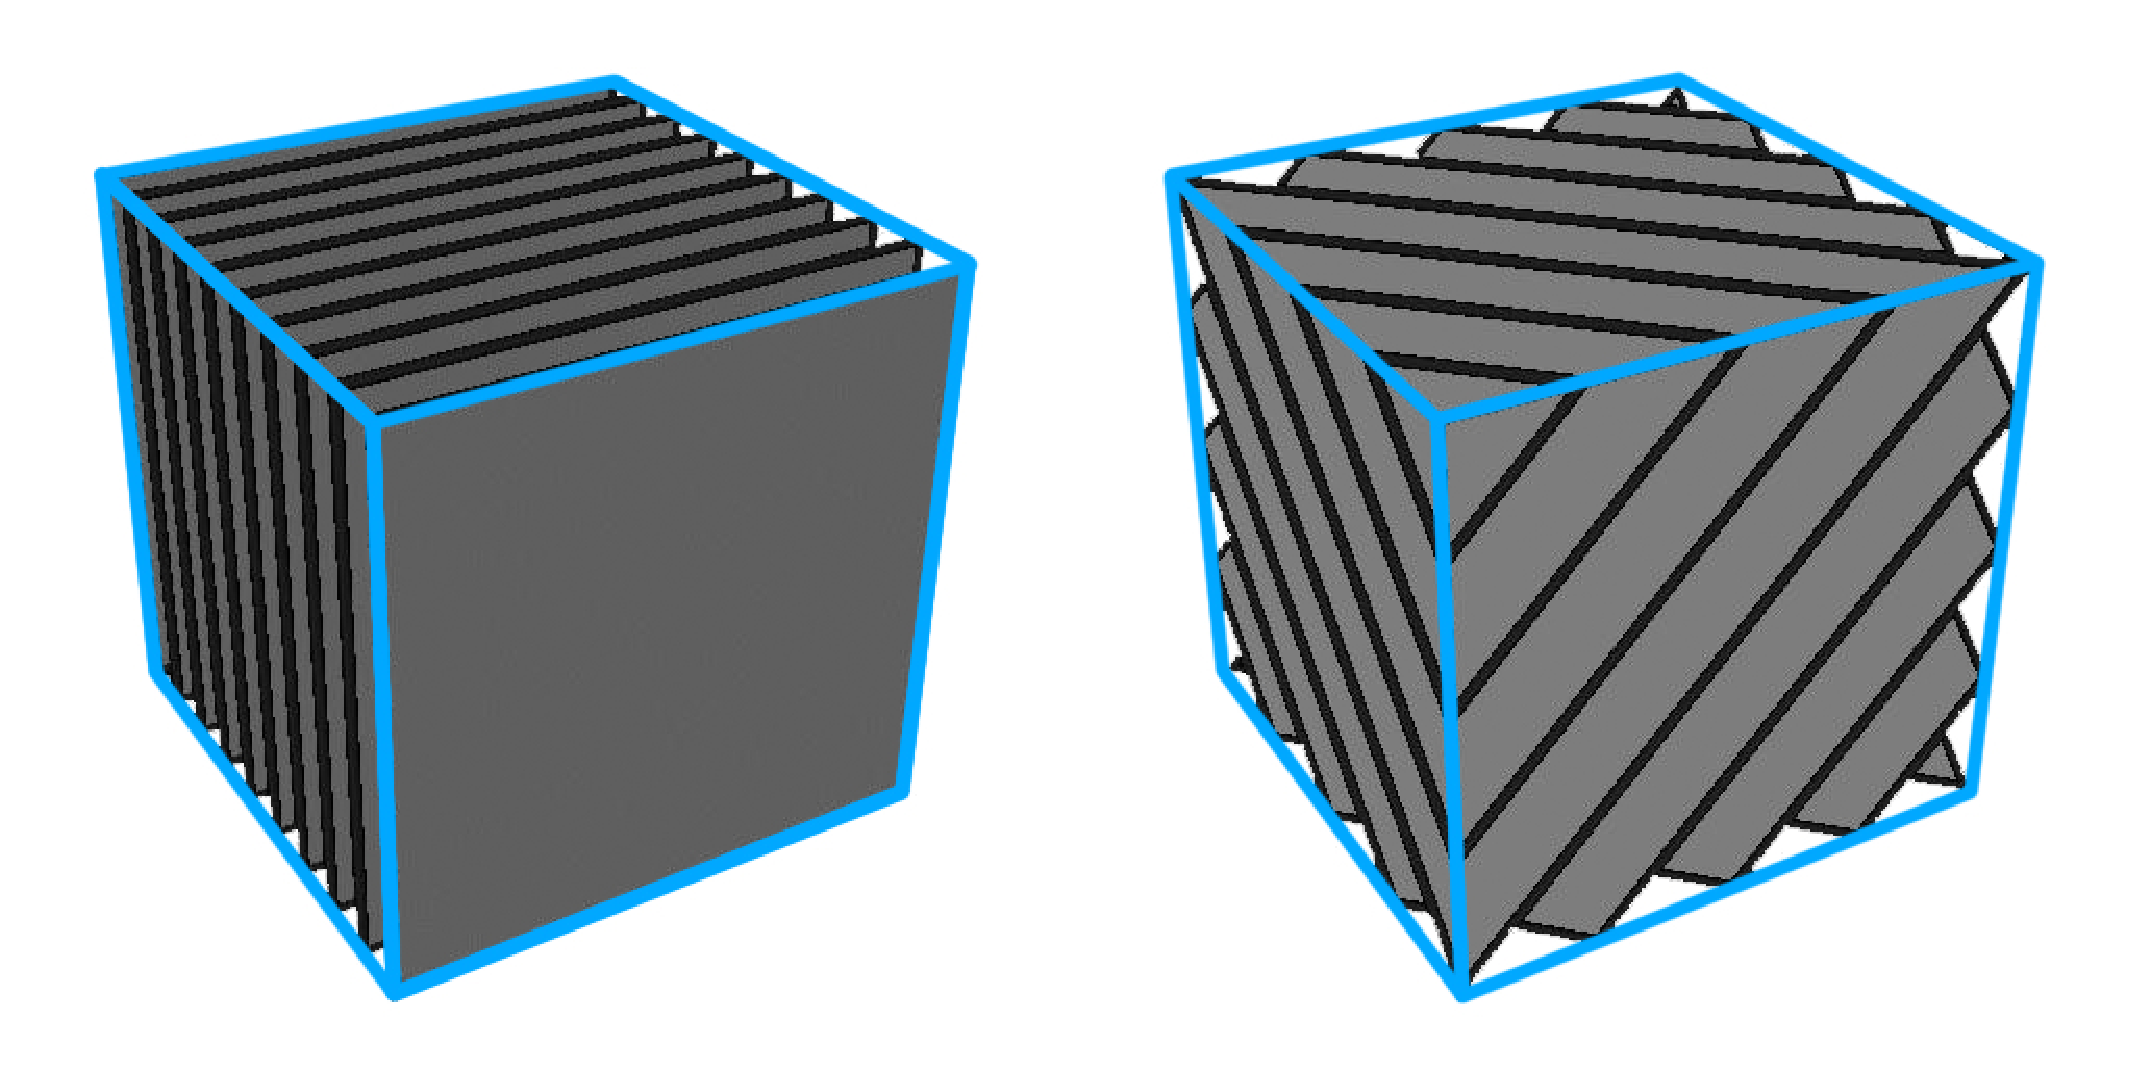
\includegraphics[width=0.7\linewidth]{images/texture_2d3d.pdf}
	\caption{Links: Texturen beim werden entlang des Volumens ausgerichtet. Recht: Texturen werden entlang des Blickwinkels ausgerichtet.}
	\label{img:2D3DTex}
\end{figure}

\begin{figure}
	\centering
	%https://www.researchgate.net/figure/Object-aligned-slice-stacks-with-2d-texture-mapping_fig1_226214561
	\includegraphics[width=0.7\linewidth]{images/textureStacks.png}
	\caption{Texturen werden als Stapel in der 	XY-, YZ- und XZ-Ebene angeordnet.}
	\label{img:textureBased}
\end{figure}

Liegen die Daten als 3D-Texturen vor, verlaufen die Querschnitte entlang der Sichtachse. Dazu werden sogenannte Proxy Geometrien erzeugt, Polygone, die einen Querschnitt beschreiben. Auf diesen Proxy Geometrien wird dann die Textur erstellt, indem die entsprechenden Volumendaten abgefragt werden. Dadurch, dass die Querschnitte an der Sichtachse ausgerichtet sind, ist nur ein Texturstapel notwendig. 


https://dl.acm.org/citation.cfm?id=329138

// TODO:
implementierung auf der grfikkarte mit 2d texuren nachteil: nur flächen nicht geometrie
3d texure based? 	
kann man shaden?

\subsection{Shear-Warp}

Shear-Warp verfolgt den selben Ansatz wie das Ray-Casting. Anstatt die Strahlen allerdings von der tatsächlichen Kameraposition aus zu verschießen, werden die Strahlen orthogonal zu den Volumenschichten in das Volumen gefeuert. Auf diese Weise wird die Berechnung der Strahlen und die Komposition der Darstellung deutlich beschleunigt. 
Damit auch bei einem nicht orthogonalen Blickwinkel das Volumen korrekt dargestellt wird, wird vor dem Ray Casting eine vom Blickwinkel abhängige Scherung auf die Volumendaten angewandt. In Abbildung \ref{img:shearwarp} ist Dargestellt, wie die Scherung die einzelnen Schichten entsprechend des Blickwinkels verschiebt, um einen orthogonalen Einfallswinkel zu simulieren. 
Das durch das Ray Casting entstandene Bild wird zunächst in einen Buffer gerendered. Durch die Scherung ist das Bild zu diesem Zeitpunkt noch verzerrt. Deshalb wird es anschließend noch einmal transformiert, sodass eine korrekte Abbildung des Volumens auf die Bildschirmebene projiziert wird. In Abbildung \ref{img:shearwarp} ist zu sehen, wie das gerenderte Bild vor und nach der Transformation aussieht. 

Shear-Warp vereint damit die Bildqualität des Ray-Castings, ist aber dabei um einiges schneller.

\begin{figure}
	\centering
	%http://citeseerx.ist.psu.edu/viewdoc/download;jsessionid=97AC0E2CDFD635B2917DF8DF86E99224?doi=10.1.1.548.9543&rep=rep1&type=pdf
	\includegraphics[width=0.7\linewidth]{images/shearwarp.png}
	\caption{Shear-Warp Verfahren. Rechts: Ohne Verschiebung würden die Strahlen der Bildebene schräg auf das Volumen treffen. Mitte: Die Schichten des Volumen werden verschoben, sodass die Strahlen orthogonal darauf treffen. Das resultierende Bild ist verzerrt. Rechts: Das verzerrte Bild wird transformiert, um das Volumen korrekt darzustellen.}
	\label{img:shearwarp}
\end{figure}

%-------------------------------------------------------------
\section{Beispiele für Volume Rendering Implementiertungen}
%-------------------------------------------------------------

Volume Rendering Techniken werden von verschiedenen Programmen und Arbeiten zur 3D-Vosualisierung von MRT-Daten eingesetzt.

Beispielsweise nutzt die kostenpflichtige Unity-Erweiterung Volume Viewer Pro Volume Ray Casting zur Darstellung von 3D-Daten. Die Anwendung ermöglicht dem Nutzer weiterhin das Erstellen eine Transferfunktion über eine Benutzeroberfläche, um das Volumen zu kolorieren, sowie das Hervorheben von Bereichen durch ein Overlay, das Laden von NIfTI- und DICOM-Dateien und einige weitere Manipulationsmöglichkeiten. 
\citet{volumeViewerPro}
Ein weiteres Unity-Plugin, dass Volume Rendering ermöglicht ist \citet{volumeRenderingUnity}. Auch hier wird Volume Ray Casting verwendet und der Nutzer kann die Farbgebung der Rendering über eine Transferfunktion beeinflussen.


%-------------------------------------------------------------
\section{Oberflächen Generierung (Weitere Methoden zur dreidimensionalen Darstellung von MRT-Daten)}		 %
%-------------------------------------------------------------
% Bsp
Wie in Kapitel \ref{motivation} beschrieben wurde, bietet eine 3D-Darstellung von MRT-Bildern einige Vorteile gegenüber einer Betrachtung der Daten in 2D. 
% Kann man das belegen?
Auf Grund dieser Tatsache gab es im Laufe der Zeit verschiedene Ansätze zur Umsetzung einer dreidimensionalen Darstellungsweise. 
Im Folgenden werden diese erläutert. 

% Vor- und Nachteile Tabelle?


\subsection{Marching Cubes}
\label{marchingCubes}
%https://developer.nvidia.com/gpugems/GPUGems3/gpugems3_ch01.html

Das Marching Cubes Verfahren wird eingesetzt, um eine Polygonenoberfläche zu erzeugen, die ein volumetrisches Objekt visualisiert. 
Der Visualisierung liegen Volumendaten, die in Form eines Skalarfeldes vorliegen zu Grunde.
Die Idee hinter dem Algorithmus ist, dass es zwischen den Voxeln, die innerhalb und außerhalb eines Objektes liegen eine Grenze gibt, die die Oberfläche des Objektes bildet. Diese Grenze gilt es zu finden. 
Die Werte der Voxel, werden dabei als Dichtewerte angesehen. Voxel innerhalb der Grenze haben eine Dichte, die außerhalb eine andere. Demnach kann ein Schwellenwert definiert werden, der die beiden Wertebereiche voneinander trennt.
Um die Grenze zwischen den Voxeln zu ermitteln, werden diese zunächst in Würfel aufgeteilt, woher auch der Name des Verfahrens stammt. Immer vier benachbarte Voxel bilden dabei einen Würfel.  

Die Vorstellung einer Grenze zwischen den Voxeln lässt sich auf die Würfel übertragen. Dabei liegt dann ein bestimmter Teil der Würfel des Volumens mit allen Eckpunkten innerhalb und ein bestimmter Teil außerhalb des Objektes. Diese Würfel liegen nicht auf der Grenze und alle ihre Eckpunkte haben jeweils ähnliche Werte. Andererseits gibt es Würfel, durch die die Grenze verläuft. Die Eckpunkte dieser Würfel können sich in ihren Werten stark unterscheiden, da jeweils ein Punkt zum Inneren und ein anderer zum Äußeren des Objektes gehören kann. 

Um also die Oberfläche zu erzeugen, die das gesamte Volumen aufteilt, wird jeder Würfel zuerst einzeln betrachtet und es wird ermittelt, ob und wie die Polygonfläche diesen einzelnen Würfel aufteilt.  Da diese Teilung auch einzelne Eckpunkte betreffen kann, setzt sich diese Oberfläche aus dreieckigen Polygonen zusammen. ?

Die Anzahl an Möglichkeiten einen Würfel aufzuteilen lässt sich errechnen. Für jeden der acht Eckpunkte des Würfels gilt eine von zwei Möglichkeiten: Entweder befindet er sich unter der Oberfläche und damit im Objekt oder eben nicht. Demnach ergeben sich für alle Punkte zusammen $2^8=256$ mögliche Fälle der Aufteilung. \cite{aigner07} Durch in Betracht ziehen von Symmetrie, könnten diese auf 15 verschiedene Möglichkeiten reduziert werden, die in Abbildung \ref{img:marchingCubes} dargestellt sind. Der Fall, dass die Eckpunkte gar nicht getrennt werden ist dabei berücksichtigt. 

\begin{figure}
	\centering
	%https://en.wikipedia.org/wiki/Marching_cubes#/media/File:MarchingCubes.svg
	\includegraphics[width=0.7\linewidth]{images/MarchingCubes.png}
	\caption{Die 15 verschiedenen Möglichkeiten, wie eine Polygonfläche einen Würfel in zwei Bereiche teilen kann.}
	\label{img:marchingCubes}
\end{figure}

Bei der Implementierung des Algorithmus werden nun alle 256 Teilungsmöglichkeiten eines Würfels in einer Look-up-Tabelle gespeichert. Um auszulesen, welcher Fall auf den momentan betrachteten Würfel zutrifft, bedarf es eines Indexes. 
Der Index ist eine achtstellige Binärzahl. Sie wird ermittelt, indem für jeden der acht Eckpunkte des Würfels geprüft wird, ob er unter dem Schwellenwert liegt, der die Unterscheidung zwischen Innen und Außen definiert oder nicht. Die Ergebnisse der Prüfung, die durch 1 oder 0 repräsentiert werden, werden aneinander gefügt. Nach der Prüfung aller Eckpunkte ist so ein achtstelliger Index entstanden. 

Durch die Verwendung dieses Index und der Tabelle lässt sich so auslesen, wie die Polygone in dem Würfel liegen. Damit ist auch bekannt, auf welchen Würfelkanten sich deren Vertices befinden. Für die Erzeugung einer Oberfläche muss weiterhin die genaue Position des Vertex auf der jeweiligen Kante ermittelt werden. Dies geschieht durch lineare Interpolation zwischen den Werten der Würfel-Eckpunkte, zwischen denen die betreffende Kante verläuft. ??
Auf die selbe Weise wird für jeden Vertex der Polygone dessen Normale berechnet, indem die Normalen der Eckpunkte interpoliert werden.

Nach und nach werden so für jeden Voxel-Würfel Polygone berechnet, die in einer Liste gespeichert und schließlich gezeichnet werden.

Der Marching Cubes Algorithmus wird häufig zur prozeduralen Erzeugung von Terrain eingesetzt. In diesem Fall ist es entscheidend, wie die Dichtewerte des Volumens generiert werden. Bei der Visualisierung von medizinischen Daten, wie MRT-Bildern werden die Bilddaten als Eingabewerte genommen.

\cite{Lorensen87}

Beschleunigung durch Unterstützung der Grafikkarte??

Erweiterungen/ Abwandlungen
%https://dl.acm.org/citation.cfm?id=3264776

%https://www.researchgate.net/publication/279205507_A_BRIEF_REVIEW_OF_SURFACE_MESHING_IN_MEDICAL_IMAGES_FOR_BIOMEDICAL_COMPUTING_AND_VISUALIZATION

%-------------------------------------------------------------
\section{Vergleich der Methoden im Überblick}											 %
%-------------------------------------------------------------
\begin{table}
\centering
\begin{tabular}{lrrrr}
\toprule
Vergleich von Methoden zur 3D Darstellung von Volumendaten\\  
\midrule 
Methode & Ergebnis & Komplexität & Vorteile & Nachteile \\ 
\midrule 
Volumerisches Ray-Casting & Rendering &  & & \\
Shear-Warp & Redering & 8,20 & & \\
2D-Texturbasiertes Volume Rendering & Redering  & 10,00 & & \\ 
3D-Texturbasiertes Volume Rendering & Redering  & 10,0 & 0 &\\ 
Marching Cubes & 3D-Mesh der Bestandteile des Gehirns  & 10,00 & 0 &\\ 
\bottomrule
\end{tabular}
\caption{Description of the table}\label{volumeRenderingVergleich}
\end{table}

//TODO
Tabelle
%-------------------------------------------------------------
\section{AR und VR (MR?)}									 %
%-------------------------------------------------------------
Occluded Display 

\subsection{Augmented Reality}

Der Begriff der \textit{Augemented Reality} (AR), also \textit{Erweiterte Realität} beschreibt die Idee, dass die physisch vorhandene Welt, die einen Nutzer umgibt angereichert wird mit zusätzlichen digitalen Inhalten. Dies geschieht z.B. indem wahrgenommene Gegenstände von virtuell erzeugten Objekten überlagert werden. 
Laut \cite{azuma97} zeichnet sich eine AR-Anwendung durch folgende Eigenschaften aus:

\begin{itemize}
\item Kombiniert reale und virtuelle Realität
\item Ist in Echtzeit interaktiv
\item 3D-Objekte existieren in dreidimensionaler Realität
\end{itemize}

AR und VR verbindet eine ähnliche Geschichte. Die frühesten VR-Systeme waren nach heutiger Definition AR-Systeme.
%Geshcihte?
Auch einige AR-HMDs funktionieren mit Stereoskopie. Die eben genannten Definition lässt allerdings auch andere Systeme zu. Tatsächlich gibt es eine Vielzahl von AR-Systemen. 
Beispielsweise kann eine AR-Anwendung mit oder manche ohne einen Bildschirm konzipiert werden, der die Augmentierung darstellt. Im letzteren Fall werden dann meist Beamer o.Ä. verwendet, um die Objekte in die reale Welt zu projizieren. 
Die Mehrzahl von AR-Software verwendet wahrscheinlich allerdings Bildschirme. %Warum?
Aber auch hier gibt es verschiedene Lösungsansätze. Dies betrifft zum einen die Positionierung des Bildschirms. Dieser kann direkt vor dem Auge des Nutzers, in der Welt oder in einem tragbaren Endgerät platziert werden.
Weiterhin können Bildschirme durchsichtig oder undurchsichtig sein. Handelt es sich um einen durchsichtigen Bildschirm, wird darauf nur die Augmentierung dargestellt. Des Vorteil hierbei ist, dass der seine Umgebung größtenteils unverfälscht wahrnehmen kann. Damit ist aber gleichzeitig der Kontrast zu den nicht unbedingt realitätsnahen 3D-Objekten größer.
Bei undurchsichtigen Bildschirmen nimmt eine Kamera die Umgebung auf und gibt sie augmentiert auf dem Bildschirm aus. Diese Technik wird z.B. verwendet wenn AR-Anwendungen für Smartphones oder Tablets entwickelt werden. In Abbildung \ref{img:ARPhone} ist dargestellt, wie eine solche Anwendung auf einem Smartphone aussieht.

\begin{figure}
	\centering
	%https://commons.wikimedia.org/wiki/File:App_iSkull,_an_augmented_human_skull.jpg
	\includegraphics[width=0.5\linewidth]{images/App_iSkull,_an_augmented_human_skull.jpg}
	\caption{Eine tabletbasierte AR-Anwendung, die auf einem Marker des 3D-Modell  eines Schädels projiziert.}
	\label{img:ARMarker}
\end{figure}

Alle Techniken haben gemeinsam, dass eine Kamera Teil des Systems ist, die die Umgebung des Nutzers aufnimmt. Dadurch werden Tiefen- und Bildinformationen gesammelt. Durch die Auswertung dieser und anderer Informationen, wie z.B. GPS- oder Wlan-Daten, können 3D-Objekte korrekt mit der Umgebung in Beziehung gesetzt werden. So ist es möglich ein virtuelles Objekt auf oder hinter ein reales zu stellen. Durch ein möglichst umfassendes Verständnis des umgebenden Raumes ist es auch möglich, dass die Elemente der erweiterten Realität in der realen Welt an der richtigen Stelle platziert werden und dort auch bleiben.
Alternativ dazu können am gewünschten Ort Markierungen gesetzt werden, die das System erkennt und somit genau dort das 3D-Modell darstellen kann. Solche Marker können verschieden aussehen. Oft werden komplexe weiße Muster dafür verwendet, weil diese gut zu identifizieren und schwer zu verwechseln sind. In Abbildung \ref{img:ARMarker} ist ein 3D-Objekt zu sehen, dass auf einem Marker platziert wurde. 

Zurzeit gibt es verschiedene AR-Systeme auf dem Markt, die sich teilweise in ihrer Funktionsweise unterscheiden. Die wichtigsten sind hier aufgezählt.

Smartphones. Wie bereits erwähnt können Smartphones oder Tablets als Fenster in die erweiterte Realität dienen. Dazu kann wahrscheinlich jedes Smartphone mit Kamera genutzt werden. Es gibt verschiedene SDKs und Frameworks zur Entwicklung von AR-Apps. Dazu gehören unter anderem \textit{ARKit} von Apple, \textit{ARCore} von Google und \textit{Vuforia}.

Binoculare HMDs. Hierzu zählen HMDs, die vor jedem Auge des Nutzers einen Bildschirm platzieren und so stereoskopisch dreidimensionale Inhalte simulieren. Im AR-Bereich sind dabei die \textit{Hololens} von Microsoft sowie das Headset von Magic Leap die wichtigsten Vertreter der Technologie. Beide Geräte haben durchsichtige Bildschirme und können unabhängig von einem Rechner verwendet werden. 
An dieser Stelle sollen auch VR-Geräte, wie die HTC Vive Pro genannt werden, die durch ihre eingebaute Kamera auch die Umgebung auf ihren Bildschirmen darstellen kann. Diese kann dabei natürlich auch mit virtuellen Inhalten erweitert werden. 

Ebenfalls als HMD zu bezeichnen ist die \textit{Google Glass} von Google. Dabei handelt es sich um ein Brillengestell, dass vor einem der Augen des Nutzers einen durchsichtigen Bildschirm fixiert, auf dem digitale Inhalte dargestellt werden können. Google Glass wird momentan allerdings nur noch in großen Firmen verwendet.

// TODO:
verlgiech systeme


\subsection{Virtual Reality}

Wenn die Realität durch AR also erweitert wird, so wird sie durch Virtual Reality völlig ersetzt. D.h. der Nutzer wird von seiner realen Umgebung abgeschnitten und in eine simulierte versetzt, mit der er in Echtzeit 
interagieren kann. Dabei wird in der Regel eine möglichst hohe Immersion angestrebt. 
Im Kontext von VR bezeichnet Immersion den Effekt, dass ein Nutzer dermaßen in die simulierte Welt, die umgibt eintaucht, dass sich diese für ihn real anfühlt und Interaktionen mit ihr natürlich werden. Wie immersiv eine Anwendung ist hängt dabei von der Anwendung selbst ab, sowie auch von dem verwendeten VR-System. 

Im Laufe der Zeit wurden verschiedene Systeme entwickelt, die eine möglichst immersive Realität erschaffen sollten. 
Bereits in den 50er Jahren wurde versucht den Nutzer in das Geschehen eines Films zu versetzten, indem er von seiner realen Umgebung isoliert wurde, und seine Wahrnehmung so auf bestimmte Reize gebündelt wurde. % Referenz Sensorama
In den 1960ern wurden dann erste Versionen eines Head Mounted Displays (HMD) entwickelt. %Referenz Sword of Dmaocles -> Eigentlich AR
Dabei handelt es sich um eine Art Brille, mit zwei Bildschirmen vor den Augen, auf die simulierte Inhalte projiziert werden.
Um den Eindruck von Dreidimensionalität zu erzeugen, wird dabei das Prinzip der Stereoskopie verwendet. Hierzu werden jeweils dem linken und rechten Auge des Nutzers zwei Bilder des selben Objektes aus leicht unterschiedlichen Blickwinkeln  gezeigt. Da die Augen beim normalen Sehen ein Objekt tatsächlich aus zwei verschiedenen Winkeln wahrnehmen, werden die Bilder im Gehirn zusammengefügt, sodass der Eindruck von Tiefe entsteht. Die Bilder werden dabei auf zwei Bildschirmen direkt vor dem Auge angezeigt, vor die eine Linse gesetzt wird, um ??

Der Blickwinkel auf ein Objekt hängt dabei von der Kopfposition des Nutzers ab. Um diesem die Möglichkeit zu geben, den Kopf zu bewegen und damit den Eindruck eines 3D Objektes zu verstärken wird die Position des Kopfes getracked. Auf diese Weise können die stereoskopischen Bilder dem Blickwinkel des Nutzers angpasst werden. Dieser erhält somit das Gefühl, er könne um das dargestellte Objekt herumgehen. 

Die Bewegungsfreiheit der Nutzers war allerdings durch die damalige Technik eingeschränkt, denn das System, mit dem das HMD verbunden war, war zu schwer, um es zu tragen und deshalb fest installiert. 
In den 90er Jahren gab es deshalb Entwicklungen in eine andere Richtung. Anstatt die virtuelle Realität nur direkt vor den Augen des Nutzers darzustellen, sollte diese um ihn herum erzeugt werden. Dazu wird der Nutzer in einem abgeschlossenen Raum platziert, an dessen Wände und Boden die Umgebung des jeweiligen Szenarios projiziert wurde. Die Immersion des Erlebnisses kann gesteigert werden, indem z.B. 3D-Brillen eingesetzt werden. Sogenannte CAVE-Systeme (Cave Automatic Virtual Environment) kommen auch heute noch zum Einsatz. Da sie allerdings sehr unhandlich und in ihrer Umsetzung kostspielig sind, eignen sie sich nicht als Massenprodukt oder für private Nutzung.

Obwohl die Simulation einer virtuellen Realität oft auf die Täuschung visueller Wahrnehmung fokussiert ist, werden in vielen Systemen auch andere Sinne angesprochen, um das Erlebnis immersiver zu gestalten. Dies gilt vor allem für das Gehör. Dem Nutzer werden dabei über Lautsprecher oder Kopfhörer zur Erfahrung passende Geräusche vorgespielt.
Eine größere Herausforderung stellt die Imitation von haptischen Reizen dar. Hierzu gibt es verschiedene Ansätze. Einer der einfacheren ist es dem Nutzer bei virtuellen Berührungen Vibrationen auszusetzen, z.B. über Eingabe Medien in seinen Händen. Es gibt allerdings mehrere Konzepte, die Haptische Impulse realistischer simulieren sollen, beispielsweise durch Handschuhe aus speziellem Material. %Referenz 
Durch die Verwendung eines Laufbands, das auf die Laufbewegung des Nutzers reagiert soll die Bewegungsfreiheit innerhalb der Simulation erweitert werden. Omnidirektionale Laufbänder können sowohl zusammen mit HMD als auch CAVEs eingesetzt werden.
Über den Verlauf der Entwicklung von VR-Systemen wurde außerdem des Öfteren versucht Gerüche zu simulieren. % Referenz??

Auf die Möglichkeiten der Nutzerinteraktion in VR-Systemen wird im Abschnitt \ref{VRInteraktion} genauer eingegangen.

Heutzutage bestehen die meistgenutzten VR-Systeme meist aus einem HMD, welches über eine Kamera verfügt, Eingabemedien (z.B. Controllern), einem Trackingsystem, das die Position der ersten beiden Komponenten verfolgt und einem Computer, der die Komponenten miteinander verknüpft und auf dem die VR-Anwendung läuft. 
In Abbildung \ref{img:vive} ist das HMD und die Controller während der Nutzung abgebildet.

\begin{figure}
	\centering
	%https://sco.wikipedia.org/wiki/Virtual_reality#/media/File:Reality_check_ESA384313.jpg
	\includegraphics[width=0.5\linewidth]{images/vive.jpg}
	\caption{Ein Nutzer trägt das HMD der HTC Vive und bedient dessen Controller.}
	\label{img:vive}
\end{figure}

  
Im Folgenden sind Hersteller von VR-Systemen aufgelistet, sowie die Modelle, die derzeit auf dem Markt zum freien Verkauf stehen.

% REDO?
\begin{itemize}
\item Facebook (Oculus Rift und Oculus Go)
\item Google (Google Cardboard, Google Daydream)
\item HTC \& Valve (HTC Vive)
\item Microsoft (Microsoft HoloLens, Windows Mixed Reality)
\item Razer (OSVR Hacker Dev Kit)
\item Samsung (Samsung Gear VR)
\item Sony Computer Entertainment (PS VR)
\item Starbreeze Studios (StarVR)
\item Lenovo (Lenovo Explorer für Windows Mixed Reality und Lenovo Mirage Solo für Google Daydream)
\end{itemize}

//TODO:
Durchegehen
Vergleich der Hardware Vorteile, nachteile

TODO: 
HTC Vive und Vive PRo -> MR
%-------------------------------------------------------------
\section{Verarbeitung von MRT-Daten}						 %
%-------------------------------------------------------------
Obwohl die Darstellung von MRT-Bildern in direktem Zusammenhang mit ihrem Zweck steht, bleibt die Verarbeitung der Daten auch bei verschiedenen Darstellungsformen gleich. 

\subsection{Arbeit eines Neurologen}
Wie bereits in Kapitel \ref{motivation} oberflächlich erläutert wurde, besteht der Nutzen eines MRTs darin, dass der behandelnde Arzt einen Einblick in die betreffenden Organe (hier das Gehirn) erhält. Dazu studiert er die einzelnen Schichten des Gehirns und hält Ausschau nach Anomalien.

Im Fall von Schlaganfällen sind diese ...

Wurde eine entsprechender Bereich identifiziert, markiert der Arzt diesen auf jeder einzelnen Schicht. 
\subsubsection{Schlaganfälle auf einem MRT}

\subsection{Software in der Radiologie}
% https://www.dicomlibrary.com/meddream/md5/index.html?study=1.2.826.0.1.3680043.8.1055.1.20111102150758591.92402465.76095170
%Use Cases
%Bsp
Um eine Diagnose stellen zu können muss der Arzt die MRT-Bilder eines Patieten genau studieren. Diese Untersuchung der Daten wird digital durchgeführt. Um dem Arzt einen Einblick in den Datensatz zu geben, gibt es spezielle Anzeigeprogramme, die diesen darstellen kann und weiterhin relevante Funktionen bietet. 
  
Wie bereits beschrieben, liegen die MRT-Bilder meist im DICOM oder NIfTI Datenformat vor. Um die Dateien öffnen zu können, bedarf es deshalb bestimmter Software. Es stehen viele verschiedene Programme zur Darstellung von MRT-Bildern zur Verfügung. Und die Auswahl eines Programms hängt meist an der persönlichen Präferenz des Arztes. 
In Krankenhäusern besteht allerding in der Regel die Situation, dass die Bilder in einem Picture Archiving and Communication System (PACS) gespeichert. (Fußnote?) Dabei handelt es sich um einen Server, der unter anderem medizinische Bilddaten zentral speichert. Die Bilder werden von bildgebenden Verfahren aus z.B. der Radiologie direkt im PACS gespeichert. Von dort aus kann entweder mit speziellen Arbeitsplatzrechnern oder auch mit herkömmlichen Computern über den Browser auch die Bilder zugegriffen werden. Dies geschieht dann meistens durch einen entsprechenden Viewer, der in das PACS integriert ist. Die Speicherung und Verteilung von medizinischen Bilddaten ist oft durch den DICOM-Standart geregelt, der im Abschnitt \ref{datenformate} genauer beschrieben ist.

Die meisten Viewer Programme für MRT-Bilder, unabhängig davon, ob es sich um PACS-Viewer handelt oder nicht ähneln sich stark in den Funktionen die sie anbieten und ihrem Aufbau.

Meist können in mehreren Fenstern verschiedene Ansichten des gleichen oder unterschiedlicher Datensätze geöffnet werden. Jedes Fenster stellt dabei eine Sichtebene dar, die gleichzeitig den Querschnitt durch das Gehirn bildet. Die verschiedenen Sichtebenen können in den anderen Ansichten farblich kodiert eingezeichnet werden, damit der Arzt ein besseres Bild davon bekommt, welchen Teil des Gehirns er gerade betrachtet.
Klassischer Weise werden drei verschiedene Blickwinkel dargestellt, die an den X-, Y- und Z-Achsen ausgerichtet sind. Die Sichtebenen verlaufen dabei orthogonal zur Blickachse. Die Ebenen können entlang der Achsen verschoben werden. Auf diese Weise scrollt der Neurologe durch die verschiedenen Schichten des Gehirns. 
Bei den drei Ebenen handelt es sich um die Frontal- oder Coronalebene, die das Gehirn in vorne und hinten teilt, die Sagittalebene, die zwischen links und rechts verläuft und die Transversalebene, die eine Teilung zwischen oben und unten bewirkt.  
Bei dieser Zusammensetzung von Ebenen wird manchmal noch eine vierte Ansicht ergänzt, auf der entweder die Sagittalebene von der anderen Seite abgebildet ist oder durch das Ineinanderschieben der gerade angezeigten Schichten eine annähernd dreidimensionale Darstellung simuliert wird. 
In Abbildung \ref{img:mrtSoftware} ist die Oberfläche der XY-Viewers zu sehen, die beispielhaft die Ansichten zeigt.

Die Benutzeroberfläche bietet auch einige Interaktionen. Die wichtigsten sind dabei die, die es dem Arzt ermöglichen ein möglichst eindeutiges Verständnis vom Inneren des Gehirns zu erhalten.  Dazu zählen:

\begin{description}
\item [Scrollen durch die einzelnen Bildschichten]\hfill \\
Dies geschieht in der Regel durch die Auswahl einer der Ansichten und die Betätigung des Mausrads. 
\item [Einstellen von Kontrast und Helligkeit D]\hfill \\
adurch können schlecht sichtbare Strukturen erkennbarer gemacht werden. Das Werkzeug dazu muss in der Taskleiste ausgewählt werden. In einem separaten Fenster können die Werte dann angepasst werden. ??
\item [Heranzoomen]\hfill \\
Bestimmte Bereiche eines Bildes können vergrößert werden, um sie besser beurteilen zu können.
\item [Verschieben des Bildausschnitts]\hfill \\
Um über ein vergrößertes Bild zu navigieren, kann der Nutzer dieses anklicken und in eine Richtung ziehen. Dies ermöglicht es andere Bildteile zu untersuchen, ohne zuerst herauszoomen zu müssen.
\end{description}

Obwohl über die Taskleiste oft noch weitere Optionen zur Verfügung stehen sind diese nicht essenziell zur Untersuchung der Bilder und werden meistens nicht oder nur in geringem Umfang genutzt, wie aus den Interviews mit Neurologen hervorging.

Es gitb eine Vielzahl von Viewern dieser Art zum Öffnen oder zur Verarbeitung von MRT-Bildern, viele davon stehen kostenloas im Internet zur Verfügung. 
Zu den wahrscheinlich meist verbreitetsten gehören \cite{osirix} und \cite{horos}, für das Betriebsystem macOS. \cite{radiocafe} stellt außerdem folgende Viewer zum Gebrauch im radiologischen Kontext für Windows vor: Das kompakte und schnelle Viewerprogramm \cite{radiant}. Weiterhin \cite{prosurgical}, was sich eigentlich an Chirurgen richtet und \cite{navegatium}, ein Programm, dass auch als Windows App und somit auch für Tabletts zur Verfügung steht.
Alle der genannten Viewer besitzen die Funktion aus MRT-Datensätzen auch Volumendarstellungen zu erzeugen.

%-------------------------------------------------------------
\section{Interaktion in AR/VR}	
\label{VRInteraktion}							 %
%-------------------------------------------------------------
\subsection{Systeminterne Nutzereingaben}

VR und AR Systeme, die es heutzutage zu kaufen gibt besitzen in der Regel  eine oder mehrere Formen der Eingabe, um mit dem System zu interagieren.

Die Eingabemöglichkeiten sind dabei teilweise von der Art des Systems abhängig. 
Beispielsweise kann für Smartphone-Apps der Touchbildschirm des Gerätes für die Nutzereingabe genutzt werden. 

Theoretisch kann jedes System mit jedem Eingabemediun verknüpft werden. Dies ist allerdings für Nutzer und Entwickler mit entsprechendem Aufwand verbunden. Die Techniken, die von den derzeit erhältlichen AR und VR Systemen verwendet werden, um Nutzereingaben zu erfassen lassen sich in zwei Kategorien teilen. 
%IMMERSION
\paragraph{Controller}
Zum einen gibt es Controller, die mit dem System zusammen hergestellt werden und die der Nutzer während der Verwendung des Systems in der Hand hält. Im Fall von VR Systemen sind meistens zwei Controller vorhanden, einer für jede Hand. Diese sind jeweils mit einer Anzahl an Knöpfen oder auch Touchpads versehen, die des Nutzer bedienen kann. Im Aussehen sind sich Controller dieser Art recht ähnlich. In Abbildung \ref{img:VRController} ist der Controller des HTC Vive Systems zusehen.
Allerdings existieren auch Systeme für dessen Bedienung nur ein Controller vorgesehen ist. Ein VR-Beispiel ist die \textit{Oculu Go}, ein eigenständiges System für grafisch weniger anspruchsvolle Anwendungen. 
Auch AR-Systeme, wie die \textit{Magic Leap} oder die \textit{Hololens} besitzen nur einen Controller. Diese haben im Vergleich zu den zuerst genannten VR-Controllern deutlich weniger Eingabemöglichkeiten. Im Falle der \textit{Hololens} handelt es sich um einen flachen Kontroller, den sich der Nutzer an den Finger steckt. Indem er Druck ausübt, kann er klicken. Daneben wird nur die Position und Rotation des Clickers verfolgt, durch die der Nutzer mit dem System interagieren kann. Das Gerät stellt damit eine von zwei möglichen Eingabemethoden dar. 

\paragraph{Gesten}
Die andere ist die Steuerung über Gesten, die vor allem AR-Systeme verwenden und die zweite Kategorie darstellt.
Die in den Systemen verbaute Kamera erfasst dabei die Hände des Nutzers in ihrem Blickfeld und erkennt bestimmte Handgesten, auf die dann reagiert wird. 
Die \textit{Hololens} kann zum aktuellen Zeitpunkt zwei Hauptgesten erkennen, \textit{Boolm} und \textit{Air tap}, sowie die Bewegung der Hand. Durch die Verbindung von beidem können beispielsweise Objekte verschoben werden. In Abbildung \ref{img:hololensGestures} ist dargestellt, wie die Hololens-Gesten ausgeführt werden. 

//TODO: 
Hololens2
Die \textit{Magic Leaop} erkennt dagegen acht verschiedene Handgesten, die in \ref{img:magicGestures} abgebildet sind. 


\begin{figure}
	\centering
	%https://www.researchgate.net/figure/The-common-air-tap-gesture-used-in-the-HoloLens-application_fig2_32914899
	\includegraphics[width=0.7\linewidth]{images/hololensGestures.png}
	\caption{Handgesten, die die Hololens erkennt.}
	\label{img:hololensGestures}
\end{figure}

\begin{figure}
	\centering
	%https://next.reality.news/news/new-magic-leap-gesture-documentation-offers-insight-into-hands-will-make-its-digital-world-come-alive-0183614/
	\includegraphics[width=0.7\linewidth]{images/magicleapGestures.jpg}
	\caption{Handgesten, die die Magic Leap erkennt.}
	\label{img:magicGestures}
\end{figure}

\paragraph{Kopfposition und Blickrichtung}

\paragraph{Sprachsteuerung}
\paragraph{HMD-Knöpfe}
Schließlich besitzen in vielen Fällen auch die HMDs der Systeme Knöpfe oder Räder. Diese dienen allerdings meistens zur Konfiguration des Systems und Steuern z.B. die Lautstärke.
%Linsenabstand? Capture?

Controller
\subsection{Leap Motion}

Die \textit{Leap Motion} ist ein externes Gerät, dass die Hände des Nutzers tracked und die genauen Handbewegungen an einen Computer übermitteln kann. 
Dies funktioniert mittels Tiefeninformationen, die die in \textit{Leap Motion} eingebaute Kamera sammelt. Das Gerät wird über USB an einen Rechner angeschlossen und kann dann als unabhängiges Eingabemedium verwendet werden. Allerdings ist auch eine Verwendung in Kombination mit AR- oder VR-Systemen möglich. 
Die \textit{Leap Motion} schafft es die Handbewegungen des Nutzers verlässlich anchzuemfinden, sodass die Hände in den digitalen Raum übertragen werden können. Hier kann nun eine Interaktion mit anderen digitalen Objekten stattfinden. 

Die \textit{Leap Motion} erkennt weiterhin vier Handgesten. Diese sind \textit{Circle}, \textit{Swipe}, \textit{Tap} und \textit{Screen Tap}. Die Gesten sind in Abbildung \ref{img:motionGestures} zu sehen. 

\begin{figure}
	\centering
	%https://developer-archive.leapmotion.com/documentation/v2/csharp/devguide/Leap_Gestures.html
	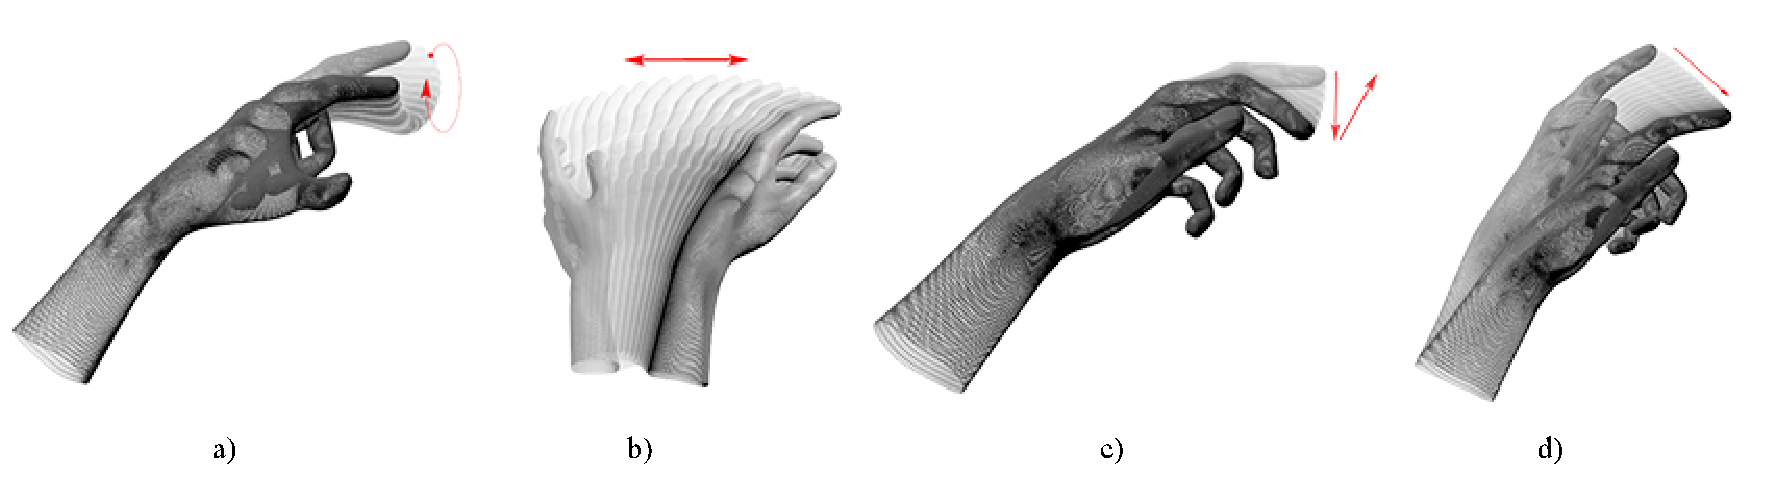
\includegraphics[width=0.7\linewidth]{images/motionGesture.pdf}
	\caption{Handgesten, die die Leap Motion erkennt. \textit{Circle} (a), \textit{Swipe} (b), \textit{Tap} (c) und \textit{Screen Tap} (d).}
	\label{img:motionGestures}
\end{figure}


\subsection{Andere}
Consolen Controller
\subsection{Interaktionsdesign}

//TODO:
Paper zur interaktion finden
-> was ist gut zur interaktion inAR warum?

\section{AR und VR im Vergleich}

Nachdem die AR- und VR-Systeme vorgestellt wurden, sollen die beiden Technologien an dieser Stelle verglichen werden.

\begin{tabular}{lrr} 
\toprule
Vergleich AR und VR\\  
\midrule 
Technologie & Vorteile & Nachteile\\ 
\midrule 
AR & Unabhängig von anderen Geräten & Eingeschränkte Interaktionsmöglichkeiten\\
   & Bewegungsfreiheit				& Entwicklung an Hersteller gebunden\\
   & Be								& Begrenzte Leisutung\\
   & Interaktion mit Umwelt möglich & Langes Tragen unkomfortabel\\
   & 								& Eingeschränktes augmentiertes Sichtfeld\\
VR & Leistungfähigkeit nur durch Rechner beschränkt  & Totale Abkapselung von der Umwelt \\
	& Kann auch kabellos verwendet werden		  	 & Langes Tragen unkomfortabel\\
	& & \\
\bottomrule
\end{tabular}







% Anforderungsanalyse

\chapter{Anforderungsanalyse}
\label{anforderung}

\section{Interviews}

Zur Bestimmung der Anforderungen, die von der Anwendung erfüllt werden sollen wurden iterativ mehrere Interviews mit dem betreuenden Radiologen der Charité geführt.


Im Rahmen des ersten Interviews wurde zunächst der Nutzen der Anwendung beschreiben.
Diese soll Neurologen im Bereich der Schlaganfallprävention unterstützen. Wie im Kapitel Grundlagen beschrieben untersucht der Neurologe dabei die Abbildungen des Gehirns eines Patienten, die durch den MRT-Scan erzeugt wurden. Auffällige Bereiche, die auf einen Schlaganfall hindeuten könnten werden dabei markiert. 
% Bezug zu Kapitel Grundlagen
Diese Darstellung soll nun inklusive des markierten Bereichs dreidimensional dargestellt werden. Durch die zusätzliche Dimension soll sowohl für Ärzte als auch Patienten die Ausmaße des betroffenen Bereich verdeutlichen, was die Einschätzung eines Schlaganfallpatienten verbessern könnte.
Weiterhin könnte man anhand des Modells auch Voraussagen von Therapieerfolgen anschaulich demonstrieren.
% Bezug zu Kapitel Motivation

Die Anwendung soll dabei als Prototyp dienen, die die Möglichkeiten, sowie das Potential für die Verwendung in der Praxis testet. Im Vordergrund steht hierbei die Darstellung in 3D, inklusive des markierten Bereichs.

Aus dem ersten Interview ließen sich außerdem folgende Anforderungen ableiten:
Die aus dem Interview ermittelten Anforderungen wurden in der folgenden Tabelle aufgelistet. Zur besseren Referenzierung wurden sie jeweils mit Bezeichner versehen. Weiterhin wurde die Priorität jeder Anforderungen auf niedrig, mittel, oder hoch geschätzt.

\begin{table}
\begin{tabular}{|c|p{10cm}|c|}
\hline
Anforderungsbezeichnung & Anforderung & Priorität \\
\hline
A01 & 3D Darstellung der MRT Daten & hoch\\
\hline
A02 & Einblenden des gekennzeichneten Bereichs  & hoch\\
\hline
A03  & 3D-Darstellung des Gehirns, die auch Schlaganfallsbereich in 3D Erkennbar werden lässt  & hoch\\
\hline
A04 & Scrollen durch Schichten der 3D-Darstellung auf mindestens einer Achse& mittel\\
\hline
A05 & Erkennbarkeit der Struktur inneren Struktur des Gehirns (entsprechend der MRT-Bilder) & hoch\\
\hline
A06 & Scrollbare 2D Darstellung der MRT-Bilder auch mindestens einer Achse & mittel\\
\hline
A07 & Manipulation der Darstellung ähnlich wie bei einem Hologramm. & niedrig\\
\hline
A10 & Interaktionselemente sollten die Darstellung nicht verdecken & niedrig\\
\hline
A11 & Scrollen durch Verwendung eines Scrollrads & niedrig\\
\hline
A12 & Auswahl verschiedener MRT-Sequenzen (falls vorhanden) & niedrig\\
\hline
A13 & Unterstützung von nifti-Daten & mittel\\
\hline
A14 & Verschiedene Ansichten können nebeneinander dargestellt werden. (z.B. vor und nach Therapie) & mittel\\
\hline

\end{tabular}
\caption{\label{tab:table-name} Durch Interview bestimmte Anforderungen.}
\end{table}

Anhand dieser Anforderungen wurden User Stories formuliert. 
%Referenz User Stories

\begin{table}
\begin{tabular}{|c|p{10cm}|c|}
\hline
Story-Bezeichnung & User Story & Anforderungsreferenz \\
\hline
U01 & Als Nutzer möchte ich ein 3D-Modell des gescannten Gehirns sehen, um ... & A01\\
\hline
U02 & Als Nutzer möchte ich den gekennzeichneten Bereich innerhalb des Gehirn sehen können, um einzuschätzen wie groß der Bereich tatsächlich ist.  & A02\\
\hline
U03  & Als Nutzer möchte ich den gekennzeichneten Bereich ein- und ausblenden können, um mich auf diesen, oder die Darstellung an sich konzentrieren zu können.  & A02\\
\hline
U04 & Als Nutzer möchte ich auch dann noch die Strukturen des Gehirns erkennen, wenn der gekennzeichnete Bereich eingeblendet ist. & A03\\
\hline
U05 & Als Nutzer möchte ich eine möglichst genaue und gut erkennbare Abbildung der MRT-Bilder, damit ich eine Vorstellung habe, wie das Gehirn des Patienten aussieht. & A05\\
\hline
U06 & Als Nutzer möchte ich durch das 3D-Modelll scrollen können, um es vergleichbar mit der 2D Darstellung zu verwenden. & A04\\
\hline
U07 & Als Nutzer möchte ich die MRT-Darstellungen frei im Raum bewegen können, um sie meiner Position im Raum anzupassen. & A07\\
\hline
U08 & Als Nutzer möchte ich die MRT-Darstellungen skalieren können, um die Darstellung gut zu erkennen. & A08\\
\hline
U09 & Als Nutzer möchte ich die MRT-Darstellungen drehen können, um den besten Blickwinkel auf den für mich relevanten Bereich zu bekommen. & A09\\
\hline
U10 & Als Nutzer will ich, dass die Darstellung nicht von anderen Elementen verdeckt wird, damit ich sie uneingeschränkt sehen kann. & A10\\
\hline
U11 & Als Nutzer möchte ich mit einem Scrollrad durch die Darstellung scrollen können, um genaue Kontrolle darüber zu haben, welche Schichten angezeigt werden. & A11\\
\hline
U12 & Als Nutzer möchte ich alle vorhandenen MRT-Sequenzen sehen und zwischen ihnen wählen können, damit ich alle notwendigen Informationen zu dem Scan nutzen kann. & A12\\
\hline
U13 & Als Nutzer möchte ich Dateien im nifti-Format in der Anwendung verwenden können, damit ich sie nicht vorher umwandeln muss. & A13\\
\hline
U14 & Als Nutzer möchte ich aus aus verschiedenen Darstellungen wählen können, die nebeneinander angezeigt werden, um direkte Vergleiche zwischen diesen ziehen zu können. & A14\\
\hline

\end{tabular}
\caption{\label{tab:table-name}Aus Anforderungen abgeleitete User Stories.}
\end{table}
% Konzept

\chapter{Konzept}
\label{konzept}

Im folgenden werden Konzepte diskutiert, um die in Kapitel \ref{anforderung} herausgearbeiteten Anforderungen zu erfüllen.

\section{3D Darstellung}

- Da das innere der 3D Darstellung erkennbar sein soll, muss eine semi-transparente Darstellung erzeugt werden, die sowohl die Form des Gehirns abbildet, als auch die innere Struktur
- Relevant sind nur die Pixel, die das Gehirn darstellen. Der Bereich darum (Schädel und Hintergrund) muss gefiltert werden. Das gewünschte Ergebniss wäre, wenn das Gehirn frei im Raum "schwebt" (Bei Ray Casting noch mal erwähnen?)

- Daten liegen dreidimensional in Schichten vor
- verschiedene Möglichkeiten zur 3D Visualisierung
- - Voxel
- - Volume Rendering (Ray Casting)
- - Marching Cubes
- - ...?

- Ist es notwendig bzw. nützlich ein  Mesh zu generieren?
	- Gut für Darstellung der Gehirnform. Relevant ist aber vor allem das "Innere" des Gehirns, da sich dort der markierte Bereich befindet. 
	- Marching Cubes eignen nich nicht, um innere Struktur Darzustellen. Eine Transparente Ansicht würde das Modell als innen "gleich" darstellen
	- Das Mesh müsste kontinuierlich angepasst werden, um jeweils andere Schichten beim scrollen anzuzeigen.
	
	- Voxel könnten auch das Innere des Gehirns darstellen. Um ein deutliches und hochaufgelöstes Modell zu erhalten währen allerdings viele Voxel notwendig. Performance?
	- Referenzen
	
	- Im Fokus der Darstellung, soll das Innere des Gehirns stehen. Ein Mesh, dass die äußere Form beschreibt ist also nicht sinnvoll, zumal keine der Anforderungen Funktionen beschreibt, für die ein Mesh nötig wäre (z.B. Kollsion (Unity))
	
Wie in dem Kapitel \ref{related} beschrieben, gibt es bereits viele Lösungsansätze zur 3D Darstellung von MRT-Bildern. Obwohl verschiedene Methodne zum Einsatz kommen, ist der am weitesten verbreitete Ansatz der des Volume Rendering.
Dies hat die folgenden Gründe:
- 
- ...
	
Diese Vorgehensweise ist somit am besten für die Implementierung der Anwendung geeignet.
Diese wird im Kapitel \ref{implementierung} genauer beschrieben.

Anforderungen an Shader??


\section{Darstellung des gekennzeichneten Bereichs}


U02 U03  


\section{Endgerät}

- Hololens oder HTC Vive?
- Leistung
- Interaktionsmöglichkeiten
- Tragekompfort
- ...
% Bezug Hololens2?

\section{Interaktion/ UI } 

% 2D 
% UX steht im Vordergrung -> begründen warum besser als vorher!

Scrollen durch 2d Bilder:
kein Mausrad-> slide vor und zurück abhängig von armlänge
slide hochrunter recht links, schwierig, ungenau

Rad wäre gut, kleines Rad (Lautstärkeregler) ideal
aber handgelenkbewegung schwer zu tracken
deshalb: Ring, den man anfasen und drehen kann, Geräusche untermalen auswahl (Feeback)

scrollwn wird oft als swipr bewegung implementiert: ungenau zu stoppen

http://blog.leapmotion.com/designing-cat-explorer/

Manipulation: Helligkeit kontrast, Größe, Verschieben, schichten scrollen, Maske?, ...

Der Use Case (REFERENZ Vergleich) erfordert es weiterhin, dass man Bilder im direkten Vergleich nebeneinander betrachten kann. Dies gilt sowohl für die zwei- als auch dreidimensionale Darstellung der Daten. Die UseCases (REFERENZ Liste) und (REFERENZ synchon) erfordern außerdem eine Möglichkeit für den Nutzen aus den vorhandenen Daten einzelne auszuwählen , die angezeigt werden sollen, sowie die Daten jeweils gleichzeitig oder einzeln zu manipulieren. 
Die Auswahl der Datensätze, sowie die Wahl ob diese synchron manipuliert werden sollen oder nicht, sind beide nicht teil der direkten Manipulation des Bildes. Sie müssen deshalb nicht in dessen unmittelbaren Umfeld stehen und der Nutzer kann sich auf sie konzentrieren. 
Die Bedienung der entsprechenden Interaktionselemente sollte trotzdem intuitiv und schnell umzusetzten sein. 
Diese beiden optionen werden deshalb in einem Menü vereint. Dieses wird an der linken Hand des Nutzers verankert. Auf diese Weise kann es immer schnell erreicht werden und wird nicht unbeabsichtigt aus den Augen verloren. Die Interaktionselemente nutzen außerdem die Möglichkeiten der VR aus, da sie i auf einem Bildschirm nicht umsetzbar wären. 
Damit das Menü nicht wären der Verarbeitung der Bilder stört, wird es nur dann eingeblendet, wenn der Nutzer seine Handfläche Richtung Kamera dreht und diese somit ansieht. Motion Leap bietet bereits Beispiel Code, der dies umsetzt. ?
Eine besondere Herausforderung bei der Konzeption des Menüs ist es, dieses möglichst klein zu halten. Das Erfassungsfeld der Motion Leap Kamera, in dem die Hände erkannt werden ist beschränkt. Deshalb kann es bei einer Interaktionfläche, die viel Raum davon einnimmt dazu kommen, dass der Nutzer versehentlich Knöpfe betätigt. 
Um den Umfang des Menüs in benutzbaren Dimensionen zu halten wurde es auf drei Knäpfe reduziert. 
Die Liste der verfügbaren Datensätze kann darin allerdings nicht untergebracht werden. Deshalb kann sie bei Bedarf über einen der Knöpfe aus geklappt werden. 
Indem der Nutzer einen Datensatz auswählt, wird dieser auf der Bildfläche angezeigt. Die Auswahl ist auf zwei Datensätze beschränkt. Zu viele gleichzeitig dargestellte Bilder würden unübersichtlich wirken und im die Motivation hinter dem Use Case ist der direkte Vergleich zweier Bilder. Außerdem stellen mehr Bilder auch mehr Möglichkeiten dar diese in verschiedenen Kombinationen zu manipulieren. Dies hätte die Anwendung unnötig verkompliziert. 
Stattdessen wird die Synchronisierung der Manipulation über einen weiteren Knopf im Handmenü gesteuert. Dieser ist nur aktiv, wenn tatsächlich zwei Bilder angezeigt werden. Dann funktioniert er als Schalter. Indem der Nutzer in betätigt wird jeweils nur eine Benutzeroberfläche neben beiden Bildern angezeigt oder sie wird dupliziert und für jede Darstellung eingeblendet. 




% auf probleme bei der visualisierung auf Hololens hinweisen, VR App 

\subsection{Interaktion AR}

\subsection{Interaktion VR}
% Leap motion

U06  Als Nutzer möchte ich durch das 3D-Modelll scrollen können, um es vergleichbar mit der 2D Darstellung zu verwenden.

U07  Als Nutzer möchte ich die MRT-Darstellungen frei im Raum bewegen können, um sie meiner Position im Raum anzupassen.

U08 Als Nutzer möchte ich die MRT-Darstellungen skalieren können, um die Darstellung gut zu erkennen.

U09  Als Nutzer möchte ich die MRT-Darstellungen drehen können, um den besten Blickwinkel auf den für mich relevanten Bereich zu bekommen. 

U10  Als Nutzer will ich, dass die Darstellung nicht von anderen Elementen verdeckt wird, damit ich sie uneingeschränkt sehen kann. 

U11  Als Nutzer möchte ich mit einem Scrollrad durch die Darstellung scrollen können, um genaue Kontrolle darüber zu haben, welche Schichten angezeigt werden.

U12  Als Nutzer möchte ich alle vorhandenen MRT-Sequenzen sehen und zwischen ihnen wählen können, damit ich alle notwendigen Informationen zu dem Scan nutzen kann.  

U14  Als Nutzer möchte ich aus aus verschiedenen Darstellungen wählen können, die nebeneinander angezeigt werden, um direkte Vergleiche zwischen diesen ziehen zu können.


\section{Unterstützung von Dateiformaten} 

Die User Story U13 verlangt nach einer Unterstützung des nifti-Dateiformats.

nifti-Dateien, sind Bilddateien, die oft in der Medizin verwendet werden. Sie speichern Bildsequenzen und eigenen sich somit für MRT-Bilder. 
% Referenz nifti
Ein weiteres für diesen Zweck weitverbreitetes Dateiformat ist DICOM. ...
% Referenz DICOM

Es ist weiterhin sinnvoll gängigere Dateiformate, wie JPEG oder PNG zu unterstützen. 

Wie in \ref{anforderung} beschrieben, soll es sich bei mARt in erster Linie um einen Prototyp handeln. 
Der Datensatz, der dargestellt werden soll ist gering. Um die Komplexität und den Umfang der Anwendung möglichst gering zu halten kann darauf verzichtet werden, dem Nutzer die Möglichkeit zu geben, aus verschiedenen Dateitypen oder Datensätzen zu wählen. Es ist ausreichend, wenn der entsprechende Datensatz vor dem Build gewählt wird.

Da die Darstellung und interaktion eines Datensatzes also im Vordergrund stehhen soll, ist es sinnvoll, die Dateien in ein Format umzuwandeln, das einfacher zu verarbeiten ist (JPEG, PNG). Hierzu kann ein externes Tool verwendet werden (ImageJ Bezug in Implementierung).

% Implementierung

\chapter{Implementierung}
\label{implementierung}

\section{Aufbau Struktur des Projektes}

Wie im Kapitel \ref{konzept} erläutert stellt mARt jeweils eine zwei- und dreidimensionale Darstellung der MRT-Daten zur Verfügung, zwischen denen gewechselt werden kann. Auf Grund der beschriebenen Hindernisse bezüglich der Leistungsfähigkeit der Hololens, wurde die Anwendung sowohl für die Hololens als auch als VR-Anwendung implementiert. Die AR-Anwendung bietet dabei nicht die volle Funktionalität und stellt die dreidimensionale Visualisierung nur beispielhaft dar. Die VR-Anwendung ermöglicht dagegen eine interaktive Echtzeit-Darstellung des Volumens. In beiden Fällen handelt es sich allerdings im Kern um die selbe Anwendung, d.h. die Software sollte für beide Gräte entwickelt werden. 
Sowohl für die Entwicklung von VR- als auch AR-Anwendungen werden im Allgemeinen GameEngines verwendet, da sie als Oberfläche diesen, um interaktive 3D-Anwendungen zu erzeugen, die in Echtzeit funktionieren. 
Zur Implementierung von mARt wurde \textit{Unity} von \citet{unity} verwendet. Die Engine gehört zu den meist genutzten auf dem Markt. Laut \citet{unityRelations} selbst, werden 60\% von AR/VR Inhalten mit Unity entwickelt. Weiterhin ermöglicht Unity die Entwicklung von Software für die meisten Plattformen. Unity bietet viele nützliche Funktionen zur Entwicklung von interaktiven Anwendungen und wird außerdem von einer großen  Gemeinschaft genutzt, sodass neben einer detaillierten Dokumentation auch über Foren und Webartikel hilfreiche Informationen zur Entwicklung zur Verfügung stehen.

Microsoft empfiehlt weiterhin Unity zur Entwicklung für Hololens-Software zu Nutzen (\citet{unityHololens}) und bietet mit \textit{Mixed Reality Toolkit} (MRTK) (\citet{holoToolkit}) ein Framework, das Hololens Funktionen innerhalb von Unity zur Verfügung stellt.
Unity verwendet C\# als Skriptsprache, was vor allem den Einstieg in die Programmierung erleichtert. Die Engine selbst ist allerdings in C++ geschrieben, wodurch effiziente Berechnungen zur Laufzeit ermöglicht werden.
%Wieso?

mARt wurde in Unity entwickelt und sollte dann sowohl für die HoloLens und als VR-Anwendung gebaut werden. Die Anwendung konnte allerdings nicht für die HoloLens bereitgestellt werden. Diese Problematik wird in Abschnitt \ref{kombination} erläutert. Auf die Entwicklung für die unterschiedlichen Plattformen wird im Abschnitt \ref{plattformen} näher eingegangen.

Um die Unity Anwendung auf dem VR-System abzuspielen, wird die \textit{SteamVR}-Software von \citep{steam} in das Projekt integriert. Um die Anwendung starten zu können muss sie auf dem jeweiligen Rechner installiert sein.

\subsection{Unity Projekt}

Unity Projekte basieren auf 3D-Szenen. Innerhalb einer Szene können GameObjects platziert werden. Dabei kann es sich z.B. um 3D-Modelle handeln. Ein GameObject besitzt verschiedene Components, die dessen Eigenschaften und Verhalten bestimmen. Viele Funktionen und Eigenschaften werden von bereits in der Engine vorhandenen Components realisiert. Sogenannte Rigidbodys verleihen einem Objekt beispielsweise physikalische Eigenschaften, die von der Engine berechnet werden. Components können auch Skripte sein, die der Entwickler selbst verfasst hat. Über diese Skripte wird die Spiellogik und die Funktionalität der Anwendung definiert. 

Da mARt sich hauptsächlich in die beiden Szenarien einer zwei- und dreidimensionalen Darstellung unterteilen lässt existiert für jedes Szenario eine Szene.
Viele der Funktionen sind allerdings ähnlich oder gleich, weshalb manche Skripte in beiden Szenen verwendet werden. 


\section{Implementierung verschiedener Technologien/Plattformen}
\label{plattformen}

\subsection{HoloLens Prototyp}
Im Rahmen der Arbeit wurde neben der endgültigen Anwendung zuerst auch eine prototypische Demo-Anwendung entwickelt, die die Hololens eigenen Gesten genutzt hat. Die Anwendung hat eine zweidimensionale Darstellung der MRT-Bilder als Hologramm in den Raum projiziert, welches der Nutzer durch Hololens eigene Gesten manipulieren konnte. Dabei wurden alle vorhandenen Manipulierungsformen eines Hologramms abgedeckt, sowie das Scrollen durch die Bildschichten. Um die Hololens Gesten zu Nutzen wurde das HoloToolkit verwendet. 
Anhand dieser Demo sollte geprüft werden, ob die Interaktionsmöglichkeiten, die die Hololens bietet ausreichend sind, um einem Neurologen die effektive Untersuchung von MRT-Bildern zu ermöglichen.
Weiterhin konnten durch das Testen einer realen Anwendung die Erwartungen und Anforderungen eines Arztes an mARt noch weiter spezifiziert werden.  

Wie im Kapitel \ref{konzept}erläutert, haben sich die Gesten der Hololens zwar als ausreichend erwiesen, machten aber die Verwendung von weiteren Bedienelementen notwendig, z.B. zum Wechseln der Manipulationsart. Aus den beschriebenen Gründen wurde für die endgültige Implementierung der Anwendung die Motion Leap in das System integriert.
% Genauer auf Implementierung eingehen

\todo{Bild von Demo}

\subsection{HoloToolkit}

HoloToolkit, Input, Camera etc
\section{Implementierung der Nutzereingabe}
Steam VR, normale scene

\subsection{Leap Motion}

Damit die Motion Leap Kamera in einer Anwendung verwendet werden kann, muss das von \citet{orion} zur Verfügung gestellte SDK \textit{Orion} eingebunden werden. Das \textit{Core SDK} ist dabei zur Erkennung und Verwendung des Gerätes notwendig, während ein erweiterndes Paket für Interaktionen die Funktionen und Beispiele bietet, wie verschiedene Bedienelemente in eine Anwendung integriert werden können, die auf die Controller, also die Hände des Nutzers reagieren.
Meistens funktioniert dies indem einzelne Skripte, die das gewünschte Verhalten implementieren als Components an GameObjects angehangen werden. Die Skripte lösen dann bestimmte Events oder Methoden aus, die mit den Funktionalitäten der Anwendung verknüpft werden. 

\subsection{Kombination von Leap Motion mit Vive/Hololens}
\label{kombination}

Sowohl Vive als auch HoloLens sollen in Verbindung mit der Leap Motion funktionieren. Dazu muss zum Einen die Leap Motion Kamera in beide Systeme integriert werden und zum Anderen die Funktionalität in die Unity jeweiligen Szenen eingebaut werden. 

Das Einbinden der Leap Motion in eine VR Anwendung, sowie die Kombination mit dem HTC Vive Headset sind unproblematisch. Das Orion SDK der Leap Motion unterstützt den Einsatz in VR-Szenen. Sofern SteamVR installiert und eine VR-Brille angeschlossen ist, ist kein größerer Aufwand nötig, um die Hände des Nutzers in VR anzuzeigen. 
Die Integration in das VR-System ist vergleichbar einfach. Die Leap Motion Kamera wird vorne auf dem HMD über der eingebauten Kamera befestigt und ihre Kabel zusammen mit den anderen der Brille über den Kopf des Nutzers geführt. 

Dagegen bringt die Verbindung von Motion Leap und Hololens einige Herausforderungen mit sich. Zunächst ist in einer Hololens-Szene nur eine Kamera, die des HMDs, vorgesehen. Das Vorhandensein einer zweiten Kamera, wie die der Leap Motion würde beim Erstellungsprozess zu Fehlern führen,sodass das Bereitstellen des Programmes für die Hololens nicht möglich ist.
Die Leap Motion wird über ihr Kabel mit Strom versorgt. Sie kann also im Gegensatz zu der Hololens nicht kabellos funktionieren. 
Über das Kabel werden außerdem die von der Leap Motion Kamera erfassten Daten weitergeleitet, die dann verarbeitet werden. Die dafür notwendige Software ist nicht für die Hololens verfügbar und es ist fragwürdig, ob sie die dafür notwendige Rechenleistung besitzt. 

Aus diesen Gründen muss die Leap Motion während des Betriebs per Kabel mit einem Rechner verbunden sein. Um das Gerät trotzdem in Verbindung mit der Hololens nutzen zu können, müssen entweder die Sensordaten der Leap Motion an die Anwendung in der Hololens übertragen werden oder die gesamte Anwendung läuft auf dem Rechner und wird zur Wiedergabe an die Hololens übermittelt. Beides geschieht über Wlan.

Die Übertragung der Sensordaten ist dabei um einiges aufwändiger und erfordert die Integration weiterer Tools. Es existieren einige Lösungsansätze für dieses Problem, beispielsweise von \citet{hololensGithub}. Auf Grund des beschränkten Zeitraums dieser Arbeit wurde dieser Ansatz allerdings nicht implementiert.
Stattdessen wird die Anwendung lediglich auf der HoloLens wiedergegeben. Dazu wird die Hololens-App \textit{Holographic Remoting Player} von \citet{remoteApp} genutzt. Die Anwendung wird dabei direkt aus dem Unity-Editor übertragen.
Die Wiedergabequalität der Anwendung ist dabei abhängig von der Stabilität der Wlan-Verbindung.

Auch das Anbringen der Leap Motion an das HMD ist bei der HoloLens umständlicher als bei der HTC Vive. 
Da es die Vive einen undurchsichtigen Bildschirm besitzt, kann die Leap Motion Kamera einfach vorne auf der Brille befestigt werden. Die Form des Gerätes bietet dazu ausreichend Fläche.
Bei der HoloLens sollte der Bildschirm, durch den der Nutzer sieht nicht verdeckt werden. Eine Installation  im oberen Teil der Frontseite ist ebenfalls nicht umsetzbar, da dieser von den HoloLens-Kameras eingenommen wird, die die Umgebung und Nutzergesten verfolgen.
Somit ist die einzige sinnvolle Möglichkeit, die Leap Motion auf der HoloLens zu platzieren. Hierbei muss sie außerdem nach vorne geneigt werden, um die Hände des Nutzers in der Anwendung möglichst genau an den realen Händen auszurichten. 
Um die Anwendung auf der HoloLens bedienen zu können, wurde eine eigene Haltungsvorrichtung gebaut.

\todo{Foto von Halterung?}


\section{Shader in Unity}

Wie in Kapitel \ref{konzept} beschrieben, wird das Volume Rendering der MRT-Daten in einem Shaders umgesetzt. An dieser Stelle soll ein Überblick über die Funktionsweise und den Aufbau von Unity-Shadern gegeben werden. 

Wie ein Objekt in einer Szene gerendert wird hängt in Unity davon ab, welches Material diesem zugewiesen ist. Das Material fungiert dabei als eine Art Behälter für sämtliche Parameter, die das Aussehen des Objektes beeinflussen, wie z.B. die Textur oder Farbe. Welche Parameter das Material besitzt und wie diese miteinander verrechnet werden bestimmt der Shader des Materials. Innerhalb des Shaders wird in Abhängigkeit zu den diesem übergebenen Werten die Farbe für jeden Pixel errechnet. 
% https://docs.unity3d.com/Manual/Shaders.html

Shader in Unity sind in der Unity eigenen Shader-Sprache \textit{Shader Lab} geschrieben. Im Shader ist definiert, welche Eigenschaften dieser besitzt und welche Sub- und Fallback-Shader er verwendet.
Die Eigenschaften sind die eben genannten Parameter, dessen Werte dann über das Material gesetzt werden. Hier werden deren Namen, Typen, ihr Wertebereich, sowie ihre Standardwerte definiert. 

Schließlich werden im Shader auch sogenannte Subshader definiert, die den eigentlichen Shader-Code enthalten.
Ein Shader kann mehrere Subshader enthalten für den Fall, dass einer der Shader von einem Gerät nicht unterstützt wird. Wird keiner unterstützt wird der Fallback-Shader verwendet. 
Neben dem Shader-Code besitzt ein Subshader Tags, die bestimmen, wann und wie ein Shader von der Rendering Engine gerendert werden soll. Dies kann sich beispielsweise auf die Reihenfolge beziehen, in der Objekte gerendert werden oder ob ein Objekt Schatten werfen soll. 
Nach den Tags folgt die Definition eines \textit{Pass}. Als Render Pass wird der gesamte Prozess bezeichnet, der durchlaufen wird, um einen Pixel zu rendern. Angefangen bei der Berechnung einzelner Vertices eines Meshes über den Vertex-Shader bis zum Fragment-Shader. D.h. im Pass werden in verschiedenen Methoden die tatsächlichen Berechnungen beschrieben, die zum Aussehen jedes Pixels führen. 
Auch ein Pass kann zunächst wieder Tags enthalten, die bestimmen wann oder wie oft ein Pass durchlaufen werden soll. 
% Render setup ????
Dann folgt der Code Abschnitt, der den Shader-Code enthält. Dieser ist in Cg (C for Graphics)
\todo{REFERENZ} geschrieben, einer Shading-Sprache, die syntaktisch stark HLSL (High-Level Shading Language) ähnelt. 
Abhängig davon, um welche Art von Shader es sich handelt werden hier die notwendigen Funktionen implementiert. Unity besitzt sogenannte Surface-Shader, ein vereinfachter Shader, für den kein Beleuchtungsmodell implementiert werden muss. Andererseits können auch Vertex-Fragment-Shader implementiert werden, die auch Unlit-Shader heißen. 

Das Volume Rendering der MRT-Daten erfolgt durch einen Vertex-Fragment-Shader auf die genaue Implementierung wird im Folgenden eingegangen. 

% https://docs.unity3d.com/Manual/SL-Shader.html
\todo{
-Was is cg hlsl?
- Was sind compute, surface, unlit shader?
- Graphic pipeline?
REFERNZEN
}
\section{Grundlage}

Die in Kapitel \ref{anforderung} beschriebenen Anforderungen stellen den Umfang der zu implementierenden Anwendung dar. 
Neben der Umsetzung der Anwendungslogik stellt vor allem die Implementierung der 3D-Darstellung durch Ray-Casting einen hohen Aufwand dar. Um diesen in einem realisierbaren Rahmen zu halten, wurde ein bereits existierendes Programm als Basis für die zuletzt genannte Funktionalität verwendet.
Wie in Kapitel \ref{grundlagen} beschrieben wurde, gibt es bereits viele Implementierungen von Volume Ray-Casting zur Visualisierung von medizinischem Bildmaterial. 
Die dort genannten Unity-spezifischen Lösungen sind allerdings kostenpflichtig und/oder ihre Codebasis ist nicht einsehbar. Es wäre allerdings von Vorteil die Kontrolle über die Implementierung der 3D-Darstellung zu haben, um so die Möglichkeit zu haben, sie den Anforderungen entsprechend anpassen zu können.
Aus diesem Grund wurde die Open-Source-Implementierung von \citet{volumeRenderingGit} als Grundlage für die 3D-Darstellung verwendet. 
Diese wurde erweitert, um die Anforderungen an mARt zu erfüllen. 
Im Rahmen der Arbeit wurden folgende Bestandteile implementiert:

\begin{itemize}
\item Erweiterung des Shaders (Maske, Beleuchtung)
\item Umwandlung von Bilddaten in 3D-Texturen und der Berechnung ihrer Gradienten
\item Anpassung der Bedienelemente an 3D-Szene
\item Anwendungslogik
\end{itemize}
Der verwendete Code ist im Projekt markiert.
\section{Volume Rendering}

Wie in Kapitel \ref{konzept} beschrieben, wurde der 3D-Darstellung des Gehirns mit Hilfe von Volume Ray-Casting umgesetzt. 

Im Kapitel \ref{grundlagen} wurde der theoretische Vorgang dieser Technik beschrieben. Dieser Abschnitt fokussiert sich auf die Implementierung der einzelnen Schritte.

Die volumetrische Darstellung des Gehirns wird im Grunde genommen mit nur 3 Skripten erzeugt. Zuerst wird in VolumeRendering.cs das Mesh des Würfeln generiert. Hier werden auch die Parameter aktualisiert, die für das Rendering relevant sind, wie z.B. die 3D-Textur oder Farbe, sowie die Parameter, die durch die Nutzerschnittstelle manipuliert werden können. 
Die Parameter werden an den Shader übergeben, in dem das Rendering definiert ist. Der Cg-Code, der den Vertex- und Fragmentshader implementiert ist dabei in ein eigenes Script ausgelagert.
\todo{Warum?}

\subsection{Ray Casting}

Im Fragment Shader des \textit{Volume\_DiffuseWITHMask.sh} 
\todo{umbenennen} wird zunächst ein Strahl definiert, der von dem aktuell betrachteten Vertex aus von der Kameraposition in die Welt "geschossen" wird. In einem selbst definierten struct werden die maximalen und minimalen Werte definiert, aus denen sich die Eckpunkte des dargestellten Würfeln zusammensetzten. Anschließend wird geprüft, ob der Strahl den Würfel schneidet. 

%-----------Intersect-----------
%Dies geschieht indem zuerst die Inverse der Strahlrichtung ermittelt wird. Die Inverse eines Vektors $v$ ist $v^-1$ und da $v^-x=\frac1}{v^x}$, ergibt sich die Inverse des Richtungsvektors des Strahls indem $1$ durch die dividiert wird.
% AABB, axis aligend etc? intersection formula REFERENZ
Um die Schnittpunkte des Strahls zu ermitteln nimmt man an, dass die sechs Seiten des Würfels auf jeweils sechs Ebenen liegen, wobei davon zwei immer parallel sind. Zuerst werden jetzt alle Schnittpunkte des Strahls mit diesen Ebenen berechnet und dann geprüft, ob die Schnittpunkte innerhalb des Würfels liegen.
Der Würfel wird durch zwei Eckpunkte beschrieben. Da der Würfel Koordinaten von -0,5 bis 0,5 hat können wir hierfür die jeweils kleinsten und größten Koordinaten nutzen. 
Die Schnittpunkte des Strahls, mit den x-, y- und z-Ebenen ergeben sich durch das Umstellen der Formel, die einen Strahl beschreibt:

\begin{align}
p=r_{Ursprung}+t*r_{Richtung}
\end{align}

$r_{Ursprung}$ ist dabei der Ursprung des Strahls und $r_{Richtung}$ seine Richtung. $p$ ist ein Punkt auf dem Strahl und $t$ ein Parameter, der bestimmt wie weit der Punkt vom Ursprung entfernt ist.

Um die Schnittpunkte mit den Ebenen zu erhalten wird die Formel nach $t$ umgestellt:

\begin{align}
t=(p-r_{Ursprung})/r_{Richtung}
\end{align}

Für $p$ werden jeweils die beiden Eckpunkte des Würfels, die jeweils auf drei der Würfelebenen liegen, eingesetzt.
Dadurch sind insgesamt sechs $t$s und damit sechs Schnittpunkte mit den Ebenen bekannt. Zwei auf jeder Ebene. Die Entfernungen werden in den zwei dreidimensionalen Vektoren $t_{unten}$ und $t_{oben}$ gespeichert. Durch den Vergleich der t-Vektoren wird festgelegt, welcher Eckpunkt und damit welche zweier paralleler Ebenen weiter vorne liegt. 
% Was wenn Strahl parallel zur Ebene ist??
Jetzt muss bestimmt werden, ob diese Schnittpunkte sich innerhalb des Würfels befinden.
Dazu werden jeweils die x-, y- und z-Werte der t-Vektoren untereinander verglichen. Für das $t$ der näher gelegenen Ebene wird der maximale, für den weiter entfernten der minimale Wert bestimmt. Ist der Wert des näheren $t$s größer als der des entfernten, schneidet der Strahl den Würfel nicht. Andersherum tut er es.
Das Verhältnis der Schnittpunkte zueinander und wie dieses durch den Verlauf des Strahls bestimmt wird ist in Abbildung \ref{img:rayBoxHit} dargestellt.

\begin{figure}[!htb]
	\centering
	\includegraphics[width=0.9\linewidth]{images/rayBox.png}
	\caption{Zweidimensionale Darstellung, wie ein Strahl durch eine Box (links) und daran vorbei (rechts) verläuft. Die Schnittpunkte des Strahls (gelb) mit den Würfelebenen (blau) sind eingezeichnet. Der Vergleich derer Abstände zum Ursprung des Strahls (rot) zeigt, ob der Strahl die Box schneidet oder nicht.}
	\label{img:rayBoxHit}
\end{figure}
\FloatBarrier

%----------------------------------------
Die beiden t-Werte werden als $t_{nah}$ und $t_{fern}$ gespeichert.
Mit dem Ursprung des Strahls und $t_{fern}$ werden Anfang, Ende und die Länge des Strahls berechnet. Mit Hilfe der Länge kann ermittelt werden um wie weit pro Iteration am Strahl entlang gegangen werden soll. Dadurch wird der Strahl nur bis zu seinem Austritt aus dem Würfel abgetastet. 

In einer for-Schleife wird jeder Strahl nun abgetastet. In jeder Iteration wird jeweils ein Punkt betrachtet. Der Punkt verschiebt sich entlang des Strahls um die zuvor berechnete Distanz.
Für jeden Punkt werden zuerst die uv-Koordinaten berechnet.

Für die Koordinaten werden dann die jeweiliges Isowerte aus der 3D-Textur gelesen, die zuvor mit den MRT-Bildern befüllt wurde.

%---------------SAMPLE VOLUME-------------
Hierbei werden lediglich die uv-Koordinaten als Indices für die Textur verwendet. 
Der Isowert ist dabei im Alphakanal der Textur gespeichert. Da es sich nicht um eine Farbe sondern nur einen Grauwert handelt, können die anderen Farbkanäle der Textur mit dem Gradienten des jeweiligen Pixels befüllt werden. Darauf wird im Abschnitt \ref{gradienten} genauer eingegangen.

Der Isowert wird außerdem noch mit der Intensität multipliziert, die der Nutzer beeinflussen kann.
\todo{Mit ergebnis abgleichen}
An dieser Stelle wird aber auch geprüft, ob der betreffende Punkt überhaupt zu sehen ist, oder aufgrund der verschiebbaren Schichten nicht sichtbar sein sollte. 
Dazu wird zuerst der aktuell betrachtete Punkt mit der Rotationsmatrix des Modells multipliziert.
\todo{ UBERPRÜFEN Warum?}
Der Punkt wird dann mit den minimalen und maximalen x-, y-, und z-Werten der verschiebbaren Schicht verglichen. Das Ergebnis des Vergleichs wird dabei in einer Variable gespeichert. Ist der Punkt kleiner als das Minimum oder größer als das Maximum wird 0 gespeichert, ansonsten 1. 
Die beiden Werte werden anschließend mit dem Isowert multipliziert.Ist einer der Werte null, ist auch der ermittelte Isowert null, was im Alphakanal totale Transparenz bedeutet. 
Das Ergebnis dieser Berechnung wird zunächst für jedem Farbkanal zugewiesen.
%-----------------------------------------

An dieser Stelle wird über die Transferfunktion der entsprechende Farbwert aus der zugehörigen Textur gelesen. Dazu wird der Isowert als Index verwendet. Die Funktionsweise und Implementierung der Transferfunktion wird in der Sektion \ref{transfer} beschrieben.
% Bezug Transferfunktion!
Die Transferfunktion wird nur abgerufen, wenn der Isowert nicht 0 ist, da sonst die Transparenz überschrieben würde.
% Tranferfunktion bei index 0 auf 0000 setzen??
Ist die Farbe bekannt, wir der betrachtete Voxel illuminiert. Dies ist in der Sektion \ref{ilumination} beschrieben. 

Der Alphawert der so erhaltenen Farbe wird noch einmal halbiert, um die Darstellung semi-transparent erscheinen zu lassen.
% WARUM

Schließlich wird der erhaltene Farbwert mit den vorhergehenden verrechnet. Die Komposition erfolgt dabei von vorne nach hinten, da der Strahl in dieser Richtung abgetastet wird, wie folgt:
% Referenz GPU Gems

\begin{align}
\hat{C}_{i}=(1-\hat{A}_{i-1})C_{i}+\hat{C}_{i-1}
\end{align}
\begin{align}
\hat{A}_{i}=(1-\hat{A}_{i-1})A_{i}+\hat{A}_{i-1}
\end{align}

Wobei $\hat{C}_{i}$ die Farbe und $\hat{A}_{i}$ die Transparenz der Farbe des vordersten Voxels ist.
Wenn diese Farbe einen vorher definierten Schwellenwert überschreitet wird die Schleife abgebrochen. Der Schwellenwert kann vom Nutzer manipuliert werden und bestimmt die ?Helligkeit? der Darstellung.

Die Farbe wird schlussendlich noch auf einen Wert zwischen 0 und 1 festgesetzt und mit der Farbe der Maske verrechnet, die auf dem selben Weg bestimmt wurde.

\subsection{Transferfunktion}
\label{transfer}

\todo{mit ergebnis abgleichen}

Um eine Transfertextur zu erzeugen, werden zunächst zwei Key-Value-Listen definiert, in denen bestimmte Isowerte einem Farb- oder Opazitätwert zugewiesen werden. In einem vom Rest der Anwendung unabhängigen Skript wird aus diesen einzelnen Punkten eine Textur erzeugt, indem zwischen den festgelegten Werten eine Interpolation stattfindet.
\todo{welche interpolation?}
Die Textur wird dann als 2D-Textur abgespeichert. Da allein die Isowerte als Index für die Zuordnung wurden, handelt es sich eigentlich um eine eindimensionale Transferfunktion. 
Allerdings werden von Unity keine 1D-Texturen als Shader Eigenschaften unterstützt. Da die Verwendung einer 2D-Textur aber keine Nachteile aufweist, wird stattdessen eine 2D-Textur verwendet, die eine einzige Y-Koordinate besitzt. 
Die Textur wird dann über das Material an den Shader übergeben. Wie im Abschnitt \ref{transfer} beschrieben, wird die Textur dann mit Hilfe eines Index' ausgelesen.

\subsection{Illumination}
\label{illumination}

Das Volumen wird mit mit dem Phong Beleuchtungsmodell illuminiert, wodurch es mehr Plastizität erhält. Das Modell wurde bereits in Kapitel \ref{grundlagen} detailliert beschrieben. Deshalb wird an dieser Stelle nur auch die Umsetzung im Shader eingegangen.
% Referenz? warum nicht blinn?
Wie beschrieben setzt sich das Modell aus drei Komponenten zusammen: Der ambienten und der diffusen Beleuchtung, sowie der spiegelnden Reflexion. Die Komponenten werden zusammen addiert, was in die endgültige Farbe resultiert. 
Die Koeffizienten werden im Shader durch Farben repräsentiert. Der diffuse Koeffizient ist dabei der vorher aus der Transferfunktion gelesene Farbwert. Um diesen nicht durch die ambiente Beleuchtung zu verfälschen, wird er mit einem konstanten Faktor multipliziert, um eine abgedunkelte Farbe zu erhalten, die als ambienter Wert verwendet wird. Die Reflextion wird weiß dargestellt.
%Als Reflexionsexponent hat sich der Wert ?10? als am besten erwiesen.

Um die Reflexion berechnen zu können müssen außerdem der Lichtvektor und die Normale bekannt sein.
Wie bereits erläutert, wird der Gradient eines Voxels als Normale verwendet. 
Der Vektor zum Licht wird aus der in Unity eingebauten Shader-Variable \textit{\_WorldSpaceLightPos0} ausgelesen.
Unterscheidung direktionales und Punktlicht?

\subsection{Gradientenberechnung}
\label{gradienten}


Die Gradienten werden vor dem Start der Anwendung berechnet und zusammen mit den Isowerten in eine 3D-Textur geschrieben. Der Gradientenvektor wird dabei in den RGB-Kanälen gespeichert und der Isowert im Alpha-Kanal, da es sich nur um einen einzelnen Wert handelt. 

Die Berechnung der Gradienten erfolgt im selben Schritt, wie das Übertragen der Skalarwerte aus den Bilddaten in eine 3D-Textur.
Dafür werden alle Bilddateien in einem Dateiverzeichnis auf das ein vorher definierter Pfad zeigt ausgelesen und in ein Array übertragen, das der Größe der Bilder entspricht. Die dritte Dimension des Arrays wird durch die Anzahl der Bilder bestimmt. 

Entsprechend der in Kapitel \ref{grundlagen} beschriebenen Finite-Differenzen-Methode, werden durch eine Convolution die Gradienten für jeden Farbwert berechnet und ebenfalls in ein Array gespeichert.
Das Gradientenarray wird anschließend mit Hilfe eines Gauß-Filters geglättet, bevor die Werte in eine 3D-Textur gespeichert werden. 

Diese wird im Assets-Verzeichnis des Projektes abgelegt. Sie werden in der Szene referenziert, um bei Bedarf an einen Shader übergeben zu werden, der den entsprechenden Datensatz darstellt. 
% Evaluation


\chapter{Evaluation}
\label{evaluation}

\section{Vergleich mit Anforderungen}

Zunächst werden in der folgenden Tabelle \ref{tab:evaluation} die implementierten Funktionen von mARt mit den in Kapitel \ref{anforderung} aufgestellten Anforderungen abgeglichen. Die Anforderung ist dabei über die entsprechende User Story referenziert. Dazu ist angegeben, inwiefern die Anforderung erfüllt wurde, so wie eventuelle Anmerkungen. 

\begin{longtable} {p{.125\textwidth}p{.225\textwidth}p{.60\textwidth}}
\toprule
User Story & Erfüllung & Anmerkungen \\
\toprule
U01 & Erfüllt & Die Darstellung der Daten ist zu großen Teilen abhängig von diesen selbst. Die Darstellung in AR ist abhängig von den Lichtverhältnissen.\\
\midrule 
U02 & Erfüllt & Die Betrachtung aus einem Winkel ist möglich.\\
\midrule 
U03 & Erfüllt & \\
\midrule 
U04 & Erfüllt & Die Anzahl der angezeigten Datensätze ist auf zwei beschränkt.\\
\midrule 
U05 & Erfüllt & Die Daten, aus denen der Nutzer wählen kann sind fest in das Programm integriert und es kann nur aus zwei Datensätzen gewählt werden.\\
\midrule
U06 & Erfüllt erfüllt & Maximal zwei Darstellungen können gleichzeitig manipuliert werden. \\
\midrule 
U07 & Erfüllt & Die zweidimensionale Darstellung kann auf einer Achse verändert werden. Die dreidimensionale auf drei.\\
\midrule 
U08 & Offen & \\
\midrule 
U09 & Erfüllt & \\
\midrule 
U10 & Teilweise erfüllt & Manipulationen außer Skalierung und Rotation werden übernommen, sofern der Wert in beiden Szenarien existiert.\\
\midrule 
U11  & Erfüllt & \\
\midrule
U12 & Erfüllt & Eine Manipulation der Maske würde dem Nutzer eine Anpassung erlauben, wurde jedoch nicht umgesetzt.\\
\midrule 
U13 & Erfüllt & \\
\midrule 
U14 & Erfüllt & \\
\midrule 
U15 & Erfüllt & Nur bei Anzeige eines Datensatzes möglich. Temporäte Manipulation.\\
\midrule 
U16 & Erfüllt & Die position wird nicht über mehrere Sitzungen hinweg gespeichert.\\
\midrule 
U17 & Offen & Nicht umsetzbar durch Abhängigkeit von einem PC.\\
\midrule 
U18 & Offen & Keine unterschiedlichen Sequenzen standen zur Verfügung.\\
\midrule 
U19 & Offen & Datensätze sind in Anwendung integriert.\\
\midrule 
U20 & Offen & Datensätze sind in Anwendung integriert.\\

\bottomrule
\caption{\label{tab:evaluation}Erfüllung der Anforderungen.}
\end{longtable}

\section{Nutzertest}

Um die Verwendung von mARt im Bereich der Schlaganfallbehandlung zu evaluieren wurde ein Nutzertest abgehalten. 
Dabei wurden sowohl die AR- als auch die VR-Anwendung von einem Neurologen getestet. 

Ergebnisse

\section{Auswertung}
% Was ist besser als vorher? Warum?
% Fazit

\chapter{Fazit}

\section{Ein Abschnitt}


\pagebreak

\printbibliography

\end{document}
